
\newpage
\section{Anhang}
\appendix
\addtocontents{toc}{\protect\setcounter{tocdepth}{0}} % Inhaltsverzeichnis zeigt keine Anhänge

\section{Musteranmeldeformular}
\label{section-Musteranmeldeformular}
\begin{figure}[H]
    \centering
    \caption{Musteranmeldeformular von der fiktiven Person Max Müller}
    \begin{adjustbox}{height=0.85\textheight, center}
        \includegraphics{anmeldungsformular1}
    \end{adjustbox}
    \label{fig:anmeldeformular}
\end{figure}

\section{Fragebogen}
\label{section-fragebogen}
\textbf{Vor der Durchführung}
\begin{itemize}
    \item In welchem Umfang besitzen Sie Vorerfahrungen mit\textit{Schüler Online 1.0}?
    \item In welchem Umfang besitzen Sie Vorerfahrungen mit der neuen Software?
    \item Welche Probleme können bei herkömmlichen, nicht-digitalen Bewerbungen von Schülern auftreten?
    \item Wer nutzt das System hauptsächlich an Ihrer Schule?
    \item Beschreiben Sie die Ausgangssituation die vorliegt, bevor Sie die Aufgabe \glqq Bewerbung eines Schülers\grqq{} durchführen.
    \item Welche fachlichen und technischen Qualifikationen sind zur Bewältigung der Aufgabe erforderlich (Aufgabenbewältigung / Softwarenutzung)? Welche Vorkenntnisse fehl
\end{itemize}
\textbf{Unmittelbar vor der Durchführung}
\begin{itemize}
    \item Welche Arbeitsschritte sind durchzuführen?
    \item Welche Hilfsmittel sind erforderlich (für die Aufgabenbewältigung / zur Softwarenutzung)? Welche davon fehlen ggf., welche sind zusätzlich gewünscht?
    \item Welche Ergebnisse / Teilergebnisse entstehen und wie werden diese ggf. verwertet / weitergeführt?
    \item Welche wichtigen Sonderfälle müssen berücksichtigt werden? (bzw. fallen dem Benutzer spontan ein; z. B. zur Arbeitsteilung / Zusammenarbeit)
\end{itemize}
\textbf{Nach der Durchführung}
\begin{itemize}
    \item Konnten Sie die Aufgabe aus Ihrer Sicht erfolgreich und vollständig abschließen? Falls nein - was hat Sie daran gehindert?
    \item Wie effektiv unterstützt die Webanwendung Sie bei der Aufgabe?  Gab es positive oder negative Erfahrungen?
    \item Haben Sie sämtliche Inhalte der Aufgabe verstanden? Gab es Stellen, an denen Sie sich mehr Unterstützung gewünscht hätten?
    \item Gab es Schwierigkeiten oder Verwirrungen bei der Aufgabe? Wenn ja, welche?
    \item Wie verständlich waren die Rückmeldungen der Anwendung?
    \item Welche Fähigkeiten setzt die Anwendung Ihrer Einschätzung nach voraus?
    \item Wie sehr entspricht die Umsetzung in der Software der Realität?
    \item Was handhaben Sie in Ihrem Arbeitsalltag bei nicht-digitalen Bewerbungen gewöhnlicherweise anders als in der Anwendung?
    \item Was würde Sie noch daran hindern die Software in Ihrem Arbeitsalltag einzusetzen?
    \item Wie sehr erleichtert Ihnen die Anwendung ihre Arbeit?
    \item Gibt es Funktionen, die Sie in ähnlichen bzw. anderen Anwendungen genutzt haben, die Sie hier vermissen?
    \item Welche Software sollte man aus Ihrer Sicht in Schüler Online integrieren bzw. eine Schnittstelle schaffen?
    \item Welche Dokumente würden Sie gerne im Prozess ausdrucken können?
    \item Welche Dokumente würden Sie gerne einscannen wollen und beim Datensatz hinterlegen?
\end{itemize}


\section{Interviews}
\subsection{Notizen des Interviews des Gymnasiums}
\label{section-InterviewGymnasium}
In welchem Umfang besitzen Sie Vorerfahrungen mit Schüler Online 1.0? 	
- Bisher gab es 2 mal pro Jahr Schulwechsel zum Lüttfeld oder Hanse Berufskolleg. Daten einpflegen läuft gut
- Eine Person hatte Praktikum im Lüttfeld => Daher vorerfahrung, aber nicht weiter geübt.

In welchem Umfang besitzen Sie Vorerfahrungen mit der neuen Software?	
- Keine









Welche Probleme können bei herkömmlichen, nicht-digitalen Anmeldungen von Schülern auftreten?	
- Daten nicht richtig in jedweder Software eingegeben => Eltern verrechnen sich bspw. mit Einschulungsjahr
- Schüler geben falsche Daten an (Nicht aus böswilliger Absicht sondern versehentlich)
- Getrennt lebende Eltern Erzieherdaten sind falsch






Wer nutzt das System hauptsächlich an Ihrer Schule?	
- Sekreteriat









Welche fachlichen und technischen Qualifikationen sind zur Bewältigung der Aufgabe erforderlich (Aufgabenbewältigung / Softwarenutzung)? Welche Vorkenntnisse fehlen ggf.?	
- Keine besonderen fachlichen oder technischen Kenntnisse notwendig
- Alles verständlich. 
- Man muss lesen können - mehr nicht. Man wird Schritt für Schritt durch das Programm durchgeführt
- Tiefgreifendes Wissen über das Schulsystem ist nicht notwendig
 






Beschreiben Sie die Ausgangssituation die vorliegt, bevor Sie die Aufgabe "Anmeldung eines Schülers" durchführen.
- Es liegt ein Anmeldeformular vor 
    - alle Punkte müssen ausgefüllt werden (leserlich). 
    - Bei wichtigen sachen (z.B. Sprachenwahl) müssen Unterlagen eingereicht werden
    - Bei unleserlichen / fehlendem wird (insbesondere telefonisch) nachgefragt. 
- Vor Corona fand alles vor Ort statt (mit Fristen), seit Corona immer mehr digital => Dies hat sich gut bewährt => Wird weiterhin übernommen => Dies bietet den Eltern Ruhe, sie haben die Daten dort zur Hand
- Manche Eltern fangen zuhause an, laden sich das Anmeldeformular herunter und wollen die Anmeldung selber ausfüllen. Dies brechen sie aber teilweise ab und wollen es lieber persönlich machen, da sie entweder aufgeben oder doch lieber persönlich nur ihre Daten abgeben.











Zu Beginn der Durchführung:	
- Es gab hier eine Unterbrechung durch ein Telefonat
- Es war zunächst unklar, wie man in das Formular zum Erfassen von Anmeldungen kommt. Die Sekretärin hatte einen Hauptmenüpunkt ausgewählt und wurde auf eine leere Seite geleitet. Sie hätte noch eine weitere Auswahl treffen müssen und auf einen Untermenüpunkt anschließend klicken müssen. Weiterhin konnte sie nicht differenzieren, wo der Unterschied zwischen den Menüpunkten "Schüler:innen" und "Anmeldungen" bestand. Sie hatte zwar als Aufgabe eine Anmeldung zu erfassen, konnte aber mit dieser Informationslage nicht korrekt navigieren. 
- Die Menüpunkte Schülerinnen und Anmeldungen sollten besser differenziert werden => unklar, welcher Menüpunkt hier für Aufgaben verwendet wird.
- Wenn die Eltern ihr Kind anmelden wollen werden sie tendenziell eher bei der aufnehmenden Schule als bei der abgebenden Schule nach Informationen zur Anmeldung suchen. 
- Es gab in Folge einer weiteren Unterbrechung einen Hinweis der Sekretärin: Es wäre super, wenn auch Pausen im Vorgang möglich wären und die Daten nicht verfallen würden. Unterbrechungen können auch mal eine halbe Stunde oder Stunde andauern. Manchmal fängt man morgens mit einer Aufgabe an, aber kann erst mittags/nachmittags weitermachen.



Welche Arbeitsschritte sind durchzuführen?	
- Schüler suchen, Daten des Schülers und der Anmeldung erfassen und alles zugehörige.
- Es muss dem Schüler noch eine Information anschließend übermittelt werden, das wurde aber von der Anmeldung genannt.	





Welche Hilfsmittel sind erforderlich (für die Aufgabenbewältigung / zur Softwarenutzung)? Welche davon fehlen ggf., welche sind zusätzlich gewünscht?	
- Es ist grundsätzlich praktisch, wenn man direkt aus anderen Stellen Text kopieren kann. Aus E-Mails funktioniert das in der Regel super, Pdf nur teilweise. 
- Es sollte von der Anwendung ein Einfügen der Daten unterstützt werden. 













Welche Ergebnisse / Teilergebnisse entstehen und wie werden diese ggf. verwertet / weitergeführt?	













Welche wichtigen Sonderfälle müssen berücksichtigt werden? (bzw. fallen dem Benutzer spontan ein - z. B. zur Arbeitsteilung / Zusammenarbeit)
- Wechsel von anderer Schule UND Wiederholung des Jahres müssen unterstützt werden
- Es gibt Flüchtlingskinder, wo nicht alle Daten vorhanden sind
- Langfristige Beurlaubung oder ähnliches, bei dem unklar ist, in welche Klasse das Kind gehen soll
    - Fallbeispiel: Kind ist in Therapie, nimmt nicht an schule teil, Eltern ziehen um und müssen es aufgrund der Schulpflicht trotzdem an der Schule anmelden
- Diese Kinder werden in der Regel in der Klinik geschult (Abfrage der Unterichtsinhalte an Schule) mit Personal der Klinik




Während der Durchführung:		

Schüler Suche
- Es war unklar, ob der ID-Schlüssel angegeben werden muss, es wurde vermutet, dass das kein Pflichtfeld ist.
- Der Schüler-Tab wird als Schülersuche nach Namen interpretiert
- Das Feld Schüler-Id-Schlüssel war unverständlich, die Sekretärin dachte laut: "Braucht man den? Wofür ist der da? Kann man den ignorieren?"
- Die Sekretärin dachte laut: "Was bedeutet die Suche? Wo genau wird gesucht?" Laut ihr wäre hier ein Anhaltspunkt wichtig (Hinweistext)










Bildungsgang
- Hier gabe es zwischenzeitlich wieder eine Unterbrechung durch ein Telefonat
- In den Anmeldungsunterlagen muss enthalten sein, zu welchem Schuljahr die Anmeldung sein soll
- Es könnte auch das laufende schuljahr sein
- Es war unklar, warum man kann keine Klasse auswählen kann => Es wäre hilfreich, wenn laut ihr die Klassen in dem Dropdown stehen. 
- Der Jahrgang sollte angegeben werden können, es steht noch gar nicht fest, welche Klassen es geben wird => Es gibt Profilklassen (Sport, Bilingual, etc.)
- Die Klasse wure als Jahrgangsstufe interpretiert.
- Die Eltern nehmen laut der Sekretärin erfahrungsgemäß den Aufnahmestatus "Angemeldet" als Bestätigung / Nachweis, obwohl die Entscheidung über eine Aufnahme an der Schule erst intern später gefällt wird. Dies könnte ein Druckmittel sein. Der Elternwille sei im Allgemeinen sehr stark ausgeprägt.
- Vorschlag: Rubrik "in Bearbeitung" statt Warteliste
- Es müssen die Daten geprüft werden, ob die Anmeldung des Schülers auf "Aufgenommen" gesetzt werden kann
- Es würde 1zu1 durch alle Daten durchgegangen werden müssen um die Anmeldung zu bestätigen
- Wünsche der Eltern können in anderen (Anwendungsfremden) Formularen mit angegeben werden => als Hinweis (?)
- Starke Einschränkungen bezüglich der Eingabe (z.B. nur zwei Namen als Wunschklassenkameraden) im Schülersystem wären hilfreich
- Unklar, warum für die Anwendung wichtig ist, dass eine Aufnahmeberatung erfolgt ist
- Die Schule gibt bei dem Schulbeginn/Ende immer genau die Daten an, das machen allerdings nicht alle Schulen so, was für Nachweise wichtig sein kann, unter anderem für Kindergeld und weitere informationen, wie lange das Kind an der Schule war
    - Es wäre das beste, wenn die Gesetzgebung den Schulbeginn/Ende vorgibt und es so für alle Schulen gleichmäßig ist
    - Es wäre hilfreich, wenn der Schulbeginn/Ende direkt unter dem Schuljahr ist und dann der Beschulungsbeginn/Ende dort individuell angegeben werden kann. Nach Klasse, Datum unklar ist, wie man weiter soll (klick auf weiter, Aufnahmestatus wird rot)
- Die Auswahloptionen beim Aufnahmestatus-Dropdown sind gut. Es wurde "Angemeldet" ausgewählt, da das Wort eine Aufnahme suggerierte. Eine Übereinstimmung der Begrifflichkeiten mit \textit{SchILD} wäre besser
- Eine Person weiß zunächst nicht, wozu die Uhrzeit dient, die andere Person erklärt, dass in der Oberstufe unterschiedliche Startuhrzeiten vorliegen. Sie fanden die Idee eine Uhrzeit mitzunotieren generell gut sobald das Feld interpretiert wurde. 
- Es sollte eine Unterscheidung oder Markierung geben, welche Felder den Eltern sichtbar gemacht werden.
- Die Schulgliederung wird interpretiert als die Schulgliederung, welche vorher besucht wurde, es war unklar was ausgewählt werden sollte
 	


Persönliche Daten
- Intuitiv, die Hausnummer in das Feld "Straße", aber nicht in "Hausnummer" zunächst eingetragen
- Die E-Mail des Sorgeberechtigten wurde in das Feld für die Schulkindmail eingetragen
- Der Tab "Persönliche Daten" sollte vor dem Tab "Bildungsgang" erscheinen, da das auch so in \textit{SchILD} ist.
- Die Suche nach der Postleitzahl-Ort Kombination funktionierte zunächst nicht.
- Die Eingabe eines Staates wird als unnötig erachtet, da es in der Umgebung keine ausländischen Wohnorte gibt. Es wäre sonst ein Vorausfüllen des Feldes mit "Deutschland" gut.
- Die Angabe eines Ortsteiles ist gut, auch dass es keine Pflichtangabe ist
- Telefonnummer (weitere) => Wunsch an wen das geht => wird nicht gesehen, dass oben der Tab für Sorgeberechtige (?) 
- Die Telefonnummer sollte bei der Sek1 den Hinweis haben, dass die Telefonnummer der Eltern benötigt wird. Ab der Sek2 sollte man die des Schülers nehmen.               




Sorgeberechtige
- Aus der Anmeldung ist nicht ersichtlich, ob alleiniges Sorgerecht. Dies wird angenommen, da nur die Mutter angegeben ist
- Es ist wichtig, dass es einen Nachweis gibt, dass eine Person alleiniges Sorgerecht oder das beide Unterschriften vorhanden sind, damit sich nicht eine Person über die andere hinweg setzt
- PLZ und Ort => auch hier konnte zunächst nicht die gesuchte Kombination aus PLZ+Ort gefunden werden.
- Sorgeberechtige Daten sollten die möglichkeit haben, dass die Adressdaten aus den Schülerdaten übernommen werden
- Es wurde versucht bei der Adressart die Straße anzugeben. 
- Es war eher unklar, warum es ein Posfach geben kann
- Der Sorgerechtigten Prozess wurde ausversehen abgebrochen durch klick neben dem Popup. Dies führt zu Unverständnis und macht den Nutzer sauer.
- Es gab eine weitere telefonische Unterbrechung
- Nochmal der Hinweis: Die Daten sollten nicht sofort nach ein paar Minuten verschwinden, auch nach logout und danach Login sollten die vorher erstellten Daten bestehen bleiben. Hier vielleicht eine Frage nach erneutem einloggen. "Sie haben noch ungesicherte Daten, wollen sie diese weiter bearbeiten?"















Notfallkontakte
Notfallkontakte werden vom Sekretariat nicht kontaktiert für Auskunft über die Leistung, etc.	


















Migrationshintergrund
- Bin zufrieden, alles wichtige vorhanden
- Die Erfassungsmaske sollte direkt angezeigt werden, auch wenn noch nicht "liegt vor" ausgewählt wurde
- Es ist unklar wie es weiter geht













Letzte Tätigkeit
- Nach Auffassung der Sekretärin hätte die letzte Tätigkeit noch im Kontext der Bearbeitung der Schüler-Daten kommen sollen, da es sich um ergänzende Informationen zur Person handelt, nicht erst nach den Sorgeberechtigten und Notfallkontakten
- Bei nicht gefundener Schule ist es unklar wie man weiterehen soll, es wird eine Checkbox überdeckt von der Suche
- In der Schulsuche sollte die eigene Umgebung bevorzugt werden bezüglich der Sortierung (also erst diese einträge und dann der Rest von NRW/Deutschland)
- Die Schulen-Suchfunktion ist sehr speziell, hier ist die Suchfunktion von \textit{SchILD} gut, wo auch kleinere details zum Finden der Schule genutzt werden
- Bei dem Dropdown "Letze Schule" sollte nur realistische Auswahlmöglichkeiten angezeigt werden (Bei Anmeldungen für die Sekundarstufe 2 sollten bspw. keine Grundschulen gelistet werden.)
- Die Checkbox unter der Schulsuche wird ignoriert und zunächst nicht verwendet.
    - Sie sollte besser Sichtbar gemacht werden.
- Wenn die Kinder die Informationen selber ins Formular geben, dann geben diese oft nur Klasse "4" an, ohne die Information 'a','b','c','d','e', ...
- Die Daten müssen aus häufig aus Zeugnissen und anderen Dokumenten gelesen werden, da die Kinder/Eltern die Informationen entweder gar nicht oder unpassend angeben	

Bemerkungen
"Bemerkung" tab sollte wieder früher kommen 
 
Qualifikationen		

Termine		

Aufnahmeberatung		

Zusammenfassung	
- Beim Speichern tritt eine Fehlermeldung auf (Die Fehlermeldung ist sehr unklar) => Hier sollte eine Führung kommen, wo genau darauf hingewiesen wird, wo der fehler liegt und wie dieser behoben werden kann.
- am besten sollte der Fokus auf das Feld gesetzt werden, welches Fehlerhaft ist.
Suche nach der möglichkeit die geendete Anmeldung zu öffnen. Klick auf Schüler/Anmeldung häufig ohne den Unterpunkt


Aufgaben 2 und 3 
- Man müsste beim Bearbeiten einer Anmeldung sämtliche Daten nochmal gegenprüfen, damit die Validität gegeben ist. 
- Die Sekretärin hovert lediglich über das Stift Symbol, mit dessen Hilfe Sie den Schülerdatensatz bearbeiten könnte.
- Die Funktion des Buttons "Anmeldungsformular" ist zunächst unklar.
- Das Anmeldungsformular wird so interpretiert, dass es nur für die Akte ist / wird als unnötig empfunden
- Es ist unklar, warum Der Haken bei "Unterlagen" nicht ausgewählt werden kann
- Es ist unklar, wozu die Checkbox "Schüler exportiert" und die Exportfunktion dienen. 
- "Anmeldung Exportieren" wird als Export an neue annehmende Schule interpretiert
- Es ist unklar, warum die blaue formatierten Texte "Dokumente" nicht angeklickt werden können
- Es wird vertrauen in die Anwendung benötigt um eine Anmeldung anzunehmen ohne alle Daten einzeln zu prüfen
- Sollte sich ein Schulkind über logische dinge hinwegsetzen, dann sollte SO2.0 darauf hinweise, dass es Diskrepanzen in den Daten gibt 
    - Beispiel 1: Wenn eine Anmeldung an die Sekundarstufe 1 erfolgt und die letzte Jahrgangsstufe=3 ist
    - Beispiel 2: Anmeldung an Sek2 als Grundschüler
    - Beispiel 3: Datumsangaben widersprechen sich
    - Es sollte dann eine Warnung erscheinen oder sich ein Fenster öffnen, sobald man speichern möchte.

- Validierungsproblemen sollten nur eine Warnung sein, da das z.B. bei Überspringen der Klasse durchaus das richtig sein kann









Nach der Durchführung:		
Konnten Sie die Aufgabe aus Ihrer Sicht erfolgreich und vollständig abschließen? Falls nein was hat Sie daran gehindert?	
- Erfolgreich beim zweiten Anlauf
- Es sind verschiedene Fragen aufgetaucht
- Es war unklar was noch fehlt
- Reiter anordnung hat alles unersichtlich gemacht
- Hilfeoption oder ähnliches wäre praktisch
- Nicht jedes mal nach neuen Anmeldungen gucken, vielleicht sollte es Ziffern oder eine andere Hervorhebung geben, dass eine neue unbearbeitete Anmeldung vorhanden ist
- Ein Handbuch wäre gut um selber Probleme zu korrigieren











Wie effektiv unterstützt die Webanwendung Sie bei der Aufgabe?  Gab es positive oder negative Erfahrungen?	
- Positiv im vergleich zum alten SchülerOnline => bessere Struktur, übersichtlicher	
- Felder sollten direkt bei Validierungsproblemen markiert werden, so das nicht im Nachhinein alle Schritte erneut durchgeführt werden müssen










Haben Sie sämtliche Inhalte der Aufgabe verstanden? Gab es Stellen, an denen Sie sich mehr Unterstützung gewünscht hätten?	
- Nur die reinen Daten genügen nicht 

Gab es Schwierigkeiten oder Verwirrungen bei der Aufgabe? Wenn ja, welche?
- Nein (nur ob Anmeldung oder Schüler Tab, aber dies ist kein großes Problem)	













Wie verständlich waren die Rückmeldungen der Anwendung?
- Ausbaufähig, es sollte mehr Feedback geben, mit konkreten Anweisungen	









Welche Fähigkeiten setzt die Anwendung Ihrer Einschätzung nach voraus?
- Es kann jeder machen, die Begrifflichkeiten wären auch für Laien verständlich	

Wie sehr entspricht die Umsetzung in der Software der Realität? 	

- Das Erfassen der Anmeldung sollte so aufgebaut sein wie die Dokumente der Schule oder vergleichbare Software ( \textit{SchILD} ), damit man beim übertragen von Daten aus einem schriftlichen Formular nicht blättern muss und beim Kopieren aus einer Software wie \textit{SchILD} die Daten in der gleicher Reihenfolge abgefragt werden, was zu weniger Verwirrung führen würde.
- Ansonsten inhaltlich genau wie mit \textit{SchILD} => entspricht der Realität. Keine Auffäligkeiten	





Was handhaben Sie in Ihrem Arbeitsalltag bei nicht-digitalen Anmeldungen gewöhnlicherweise anders als in der Anwendung?	
Die Sekretärinnen gucken bei dem Papierformular nach, ob es irgendwo lücken gibt => Versuchen diese selber zu füllen und nehmen ansonsten Kontakt auf
- Ganz unwichtige Daten (Geburtsort) werden, falls es abgeschlossen werden muss, im notfall ausgedacht
- Wichtige Daten müssen mit Urkunden, etc. ausgefüllt werden	














Was würde Sie noch daran hindern die Software in Ihrem Arbeitsalltag einzusetzen?	
- Noch ein zusätzliches Programm => Mehr Aufwand 
- Dopplung zu \textit{SchILD} 
- Es sollte die Möglichkeit geben eine E-Mail anzugeben, wenn neue dinge (z.B. eine Anmeldung) vorhanden sind, womit dann in einem einstellbaren Intervall Neuigkeiten empfangen werden können.	
		












Gibt es Funktionen, die Sie in ähnlichen bzw. anderen Anwendungen genutzt haben, die Sie hier vermissen?
Die Filterung der Schule wie in  \textit{SchILD} , ansonsten alles bereits zuvor erwähnte.	







Welche Software sollte man aus Ihrer Sicht in Schüler Online integrieren bzw. eine Schnittstelle schaffen? 	
 \textit{SchILD} 	





Welche Dokumente würden Sie gerne im Prozess oder am Ende des Prozesses ausdrucken können?
- Die Sekretärin fand es gut dass das Anmeldeformular ausdruckbar war um es ggf. zu archivieren.
- Schweigepflichtsentbindung, Einverständnis für PKW / Bulli Mitfahrten, Fotoerlaubnis für Webseite / intern, 

Welche Dokumente würden Sie gerne einscannen wollen und beim Datensatz hinterlegen?
Keine.	


\subsection{Notizen des Interviews der Realschule}
\label{section-InterviewRealschule}
Vorab: 	
- Internet ist langsam, die Anwendung braucht anfangs lange zum Laden
- mehrere Personen haben das Sekretariat betreten, aber keine Unterbrechnung
 
In welchem Umfang besitzen Sie Vorerfahrungen mit Schüler Online 1.0? 	
- Keine				
In welchem Umfang besitzen Sie Vorerfahrungen mit der neuen Software?	
- Keine







Welche Probleme können bei herkömmlichen, nicht-digitalen Bewerbungen von Schülern auftreten?
- Falsch ausgefüllt
- Fehlende Angaben
- Nicht leserlich
- Falsche Daten
- Begriffe wie Konfession nicht verständlich, Schulformempfehlung unverständlich, bewusst falsche Angaben, Sorgeberechtigungen, negativbescheinigung oder verpflichtend 2 Sorgeberechtigte, sensible Daten




Wer nutzt das System hauptsächlich an Ihrer Schule?
Nur das Sekretariat, beide Sekretärinnen übernehmen die gleichen Aufgaben










Welche fachlichen und technischen Qualifikationen sind zur Bewältigung der Aufgabe erforderlich (Aufgabenbewältigung / Softwarenutzung)? Welche Vorkenntnisse fehlen ggf.?	
- Man muss lesen und schreiben können, nicht mal internetaffin sein.
- Man muss sehr gewillt sein es auzuprobieren		










Beschreiben Sie die Ausgangssituation die vorliegt, bevor Sie die Aufgabe "Bewerbung eines Schülers" durchführen.	
- Es steht zunächst die Frage im Raum: "Darf dieses Kind unsere Schule überhaupt besuchen?". Diese Entscheidung basiert auf der Schulempfehlung sowie Gesprächen im Voraus mit der Schulleitung
- Die Eltern füllen vorgefertigte Unterlagen nach Anmeldeformular, Rest per Post, Mail oder in Person, wenn Deutsch schwierig zusammen in Person ausfüllen	
- Anmeldeschein der Grundschulen sind farbig gedruckt, um Mehrfachanmeldungen zu vermeiden
- Mehrere Anmeldungen an unterschiedlichen Schulen fallen in der Regel spätestens bei Kennenlernterminen auf. 
 - Die Sekretärin zitiert exemplarisch fiktive Eltern: "Mal gucken wie sich das Kind entwickelt", laut Schulgesetz kann ein schulkind jederzeit abspringen	
- Eine Lösung durch Anwalt kommt immer mal wieder vor, aber meist wird sowas per Telefon geklärt
- Pessimistische Haltung gegenüber Mehrfachanmeldungen bei der Software
- Bewerbung an mehrere Schulen ist 'grauenvoll'



Zu Beginn der Durchführung:	






















(DAkkS) Welche Arbeitsschritte sind durchzuführen?
- Es wird großer Wert darauf gelegt, dass die Personen einmal vor Ort erscheinen








Welche Hilfsmittel sind erforderlich (für die Aufgabenbewältigung / zur Softwarenutzung)? Welche davon fehlen ggf., welche sind zusätzlich gewünscht?	



















Welche Ergebnisse / Teilergebnisse entstehen und wie werden diese ggf. verwertet / weitergeführt?













Welche wichtigen Sonderfälle müssen berücksichtigt werden? (bzw. fallen dem Benutzer spontan ein; z. B. zur Arbeitsteilung / Zusammenarbeit)	
- HerkunftsSprachlicherUnterricht (HSU) muss angemeldet werden, bei Schulamt (Kreis Lippe) jedes Jahr neues Anmeldeformular, muss unterschrieben werden














Während der Durchführung:
Schüler Tab
Die Sekretärin behauptet, dass sie den ID-Schlüssel natürlich nicht wissen kann und sucht unmittelbar danach nach dem Schüler.





















Bildungsgang
- Der Sekretärin fehlt das Wort 'Neuaufnahme' aus  \textit{SchILD} 
- Das Wort Warteliste bedeutet in \textit{SchILD} etwas anderes
- Die angegebene Telfonnummer ist eine unsinnige - Man würde dann bei der anderen, mobilen Nummer anrufen.
- \textit{SchILD} hat veraltete Daten von Schulen
- Es wurde festgestellt, dass das Klassen-Dropdown nicht lädt oder keine Einträge im System vorliegen, 
- Datum kann auch per Tastatur eingegeben werden -> Falsches Datumsformat wurde eingetippt
- Es ist unklar, ob der Beschulungsbeginn selbst gepflegt werden muss, Frage: "Wie lange sind die Kinder dann bei uns?"















































Persönliche Daten										
- Für uns sind Ortsteile interessant





















Sorgeberechtigte
- Im Feld Adressart wurde die Straße eingegeben.
- Die Hausnummer wurde zusätzlich im Feld Straße eingegeben




































Notfallkontakte
- Aussage "Wir geben nur noch die ein, die zusätzlich sind"
- Es wurde 'Arbeitsplatz Vater' bei Vorname eingetragen (sowie Handy Vater, Handy Mutter)
- Frage: "Wie hinterlege ich, dass es sich um den Arbeitsplatz handelt"	
- Dropback speichert nicht
- Speichern-Button wird von Dropdown verdeckt, Handynummer wurde zwischenzeitig zunächst nicht akzeptiert	
- Autocomplete-Feld wird als nicht individuell ausfüllbar wahrgenommen, Aussage: "Wenn ein Dropdown auf geht, höre ich auf zu tippen"							










Migrationshintergrund
- "Nicht vorhanden" ausgewählt und direkt weiter im Prozess navigiert.	














Letzte Tätigkeit
"letzte Tätigkeit -> also passt das 
Ansonsten könnten wir das hier eingeben
- Aussage: "Das Kind kann ja noch keinen Abschluss haben, Für uns ist die Seite sinnlos

Bemerkungen 
- Frage: "Wer kann die internen Notizen sehen?"
- Das ist das, was ich bisher immer über die Excel Liste gemacht habe' bemerkung für Schulkind, 
- Die Felder "Interne Notiz" und "Bemerkung für Schüler*in" wurden mit der Aussage "Interne Notizen sind unsere Meinung, Bemerkung ist Fakt".  kommentiert.									

Aufnahmeberatung										
- Die Termine müssen nicht ausgefüllt werden, da es ja schon eine Aufnahmeberatung gab.

Zusammenfassung
- Die Ladezeit der Seite hatte ein paar Sekunden gedauert.
- Der Wortlaut der versandten E-Mail ist wahrscheinlich kritisch formuliert, so wie die Meldung andeutet.
- Die Email sollte aussagen, dass die Anmeldung eingegangen ist, nicht dass das Kind aufgenommen wurde
- Ich habe keinen jahrgang vorliegen, auf den sich der Schüler bewerben möchte. Es ist wichtig für uns, in welchem jahrgang das Kind bei uns aufgenommen werden soll
- Die Sekretärin benötigt noch eine Unterschrift, wir müssen das ja prüfen
- Passt das Schuljahr? Wir würden bei dieser Unklarheit anrufen.

Übersichtsliste
- Man hätte es gerne auf einen Blick, was noch zu tun ist.
- Die Chat-Funktion wurde kommentiert mit "Ich möchte doch nicht mit den Schülern reden".

Aufgabe 2 + 3:
Bewerbung-Tab 'Anmeldung wurde exportiert' unklar
- Die Nachweise dürfen wir nicht schriftlich haben
- Warn die Geburtsorte der Eltern hinterlegt? -> Nein
- Speichern hat zu Fehler geführt -> Indikator an den Reitern wären gewünscht
- \textit{SchILD} wird's mir nachher sagen, wenn was falsch war
- Die meisten 5-Klässler, die sich bei uns bewerben, haben noch keine Email
- Nachweis für alleiniges Sorgerecht verpflichtend

Am liebsten hätte ich meinen eingescannten (Anmelde)-Bogen mit drin"		



Konnten Sie die Aufgabe aus Ihrer Sicht erfolgreich und vollständig abschließen? Falls nein was hat Sie daran gehindert?
- Ich konnte das abschließen.		
- Anmeldestatus ist auf angemeldet gesetzt 	



















Wie effektiv unterstützt die Webanwendung Sie bei der Aufgabe?  Gab es positive oder negative Erfahrungen?	
- Ich hab 2 mal gesagt, dass das gut ist
- Es muss jetzt in \textit{SchILD} übertragbar sein
- Iserv auch wichtig, sonst keine weiteren Schnittstellen
- Bei den Notfallkontakten hätte ich weitere Informationen benötigt.
- Die Standardinformationen, die ein Schüler einreichen muss, sollte in den Notizen erfassen vereinfacht werden (darf das Kind fotografiert werden, Sport, hat Schwimmabzeichen, etc)
- Der wird jedes Jahr neu diskutiert (?)
- Die Farben sind schön			





Haben Sie sämtliche Inhalte der Aufgabe verstanden? Gab es Stellen, an denen Sie sich mehr Unterstützung gewünscht hätten?			
- Der Jahrgang ist wichtig, direkt auf der Anmeldungen-Seite	

Gab es Schwierigkeiten oder Verwirrungen bei der Aufgabe? Wenn ja, welche?	
- Die Felder zum Export waren verwirrend. Aber wenn man es 3 mal gemacht hat gibt's bestimmt keine Probleme mehr
- Ich hätte den Speichern-Button auch nach oben gesetzt (Sorgeberechtige)			











Wie verständlich waren die Rückmeldungen der Anwendung?
- Es gab ja nur einen Anwenderfehler, sonst hat er (die Anwendung) nicht viel mit uns gesprochen			









Welche Fähigkeiten setzt die Anwendung Ihrer Einschätzung nach voraus?	
- Man braucht eine Maus, Tastatur und man muss lesen und schreiben können
- Mindestens die Grundzüge des Schulgesetzes müssen bekannt sein
- Selbst Praktikanten könnten das eingeben, es müsste dann aber geprüft werden

Wie sehr entspricht die Umsetzung in der Software der Realität? 
- Im Prinzip entspricht das 1 zu 1 der Eingabe in  \textit{SchILD} 
- Die Notizen der neuen 5er sollten in einer Liste zusammenführbar sein
- Was mir sehr gut gefällt, ist dass die Kinder informiert werden
- Das sind 4 Arbeitschritte in einem, was super ist
- Das Programm könnte der abgebenden Schule mitteilen, dass der Schüler aufgenommen wurden
- Die Sekretärin sieht Probleme mit Mehrfachbewerbungen	






Was handhaben Sie in Ihrem Arbeitsalltag bei nicht-digitalen Bewerbungen gewöhnlicherweise anders als in der Anwendung?
- Aussage: "Ich geb das direkt in \textit{SchILD} ein, ich gucke ob die Daten passen, sonst nichts"
- Die Validierung der PLZ und Orte, Kilometerangabe automatisch ermitteln, Ortsteile aus PLZ-Ort ermitteln
 - Aktuell mache ich das mit Google Maps
- In \textit{SchILD} eingeben, bei Fragen anrufen, Stammsatz ausgedruckt, in Akte ablegen. Die Lehrer präferieren die Daten in Papier, weswegen wir das ausdrucken
- Es wären weitere Daten notwendig einzugeben bei zwischenjährigen Wechsel: Welche Schulform davor besucht wurde und wie viele Jahre








Was würde Sie noch daran hindern die Software in Ihrem Arbeitsalltag einzusetzen?
- Es fehlen noch Informationen, die irgendwie erfasst werden müssen: Angaben zum Ipad müssen erfasst werden (Mietvertrag, Kaufoptionen, etc...)
- Die Email muss dafür stimmen und muss überprüft werden, kann auch gerne mal falsch sein.
- Schulbuchbestellung mit in Email an Schüler integrieren, Materialliste (Mappen, Stifte etc)
- Noten werden auch erfasst (wurde anfangs vergessen)			
- Die Geburtsurkunde muss uns vorliegen, Die Datenschutzerklärung von uns muss gelesen werden, der Impfausweis muss vorgelegt werden, darf aber nicht erfasst werden. Regulär prüft das bereits die Grundschule und hinterlässt uns eine Notiz wie "Impfbuch wurde vorgelegt" oder "Impfschutz liegt vor", dann wissen wir was gemeint ist. 





Gibt es Funktionen, die Sie in ähnlichen bzw. anderen Anwendungen genutzt haben, die Sie hier vermissen?
- \textit{SchILD}  bietet mehr Auswahl bei den Notfallkontakten			






Welche Software sollte man aus Ihrer Sicht in Schüler Online integrieren bzw. eine Schnittstelle schaffen? 	
- Iserv und  \textit{SchILD} 			
- ISERV wird verwendet, das ist eine Software über die Schulen mit anderen Schulen, Kindern etc kommunizieren (auch Termine)



Welche Dokumente würden Sie gerne im Prozess oder am Ende des Prozesses ausdrucken können?	
- Für die Schülerakte ein Schülerstammblatt und jedes Jahr die Notenübersicht			

Welche Dokumente würden Sie gerne einscannen wollen und beim Datensatz hinterlegen?	
- Alle Formulare, die für die Anmeldung relevant waren (vor allem das Anmeldeformular)			

\subsection{Notizen des Interviews der Förderschule}
\label{section-InterviewFoerderschule}
Interview mit Förderschule
In welchem Umfang besitzen Sie Vorerfahrungen mit Schüler Online 1.0? 		
- Keine

In welchem Umfang besitzen Sie Vorerfahrungen mit der neuen Software?		
- Schon einmal kurz reingeguckt, auch schon die Elternseite
- Seite war schon offen und angemeldet	
- Nur bund-ID ist möglich, für unsere Eltern wäre das zu schwer. Man müsste das simplifizieren, ein Link zum Einloggen wäre gut ohne Bund-ID
- Leichte Sprache ist sehr wichtig, sogar auf englisch
- Export zu Excel und \textit{SchILD} wäre gut.
- Einstellung "Ich probier mal lieber, als mir was anzuhören"
- Aussage: "Die (Datensätze unter Anmeldungen) sind einfach so reingekommen" (Ihr ist zu Anfang aufgefallen, dass die Daten zu Aufgabe 2 und 3 vorliegen.)



Welche Probleme können bei herkömmlichen, nicht-digitalen Anmeldungen von Schülern auftreten?
- Meistens nur, dass die (Hand-)schrift der Anmeldeformulare nicht lesbar ist, vor allem die E-Mail-Adressen
- Für die Eltern ist es meist recht entspannt, Ablauf ist Gespräch -> Mail -> Gespräch mit Rundführung -> Unterlagen ausgefüllt
- Unterlagen direkt ausfüllen geht auch
- Selten vom Schulamt direkt
- Schon recht simpel, komplizierter macht keinen Sin. (?)
- Anmeldeformulare manchmal nicht direkt aufzufinden (?)



Wer nutzt das System hauptsächlich an Ihrer Schule?
- Das Sekretariat im Zusammenspiel mit Verwaltung, 
- Trennung zwischen Lehrer und Schule Trennung Erfassen und Übernehmen in \textit{SchILD} (?)
- Es gibt mehrere Standorte	
- Die Klasseneinteilung erfolgt nach Schulbesuchsjahren, dadurch unterschiedliche Altersklassen, daher auch keine Standortunterscheidung




Welche fachlichen und technischen Qualifikationen sind zur Bewältigung der Aufgabe erforderlich (Aufgabenbewältigung / Softwarenutzung)? Welche Vorkenntnisse fehlen ggf.?
- technisch erstmal n Rechner, Internet
- wir im Sekretariat würden damit klar kommen. Einmal gesehen, damit man weiß wie das grundlegend funktioniert.
- Kenntnisse zum Schulgesetz nicht unbedingt
- Informationen werden weitergegeben an Busunternehmen etc. Die Eltern hier unterschreiben die auf dem Formular (Datenschutz)
- Also man darf nicht einfach alles eintragen. Man muss auf Datenschutzaspekte achten





Beschreiben Sie die Ausgangssituation die vorliegt, bevor Sie die Aufgabe "Anmeldung eines Schülers" durchführen.		
- Mit den Eltern haben wir schon vorher telefoniert, wir warten auf den Zettel, es muss noch ein Gutachten gemacht werden (entscheidet sich am ende des Kindergartens) es gibt unterschiedliche Arten von Gutachten
- Wir achten auf das Einzugsgebiet
- Meist reicht uns schon die Info, dass das Kind autistisch ist						















Zu Beginn der Durchführung:		


- Ist initial zum Menüpunkt "Schulkindern" gewechselt, nicht zum Menüpunkt "Anmeldungen"








Welche Arbeitsschritte sind durchzuführen?		
- Es muss geklärt werden, ob Rundgang durchgeführt wurde
- Daten müssen aufgenommen werden und das Gutachten für später in den Akten angefordert werden.
- Es muss ein kurzes Kennenlernen stattfinden
- Es muss entschieden werden in welche Klasse das Kind kommt, dann in die Struktur




Welche Hilfsmittel sind erforderlich (für die Aufgabenbewältigung / zur Softwarenutzung)? Welche davon fehlen ggf., welche sind zusätzlich gewünscht?
- Die Eltern müssen bei uns im Vergleich zu anderen Schulen mehr an die Hand genommen werden
- Google maps verwende ich sehr selten















Welche Ergebnisse / Teilergebnisse entstehen und wie werden diese ggf. verwertet / weitergeführt?		
- Am Ende werde ich drei Anmeldungen haben.
- Eine Rangfolge in der Übersichtsliste wäre gut (durchnummerriert) wie eine laufende Nummer, die sich nicht ändert. Wäre fürs für abheften sinnvoll und dann später in \textit{SchILD} übertragen







Welche wichtigen Sonderfälle müssen berücksichtigt werden? (bzw. fallen dem Benutzer spontan ein; z. B. zur Arbeitsteilung / Zusammenarbeit)		
- Einen Feste Sortierung, damit die Reihenfolge immer gleich bleibt	Anmeldung Nr1, Nr2... Ordner ausgedruckt, nach der Nummer sortiert, um die so im Büro schriftlich abzuarbeiten














Während der Durchführung:									
- Es gibt die Primarstufe, Sek I, Sek II so nicht bei uns.
- Ankreuzen, mit wem habe ich schon den Rundgang gemacht
- Eine "Schulstufe" reicht mir. Und wir würden die dann gerne nach sortieren dann die Anmeldungen nach schulkindalter sortieren.
- Sucht jetzt nach dem Kind => Suche war eigenartig	
- ID Schlüssel ist unklar



















Bildungsgang
- Die Reihenfolge der Schuljahre ist nicht sinnvoll
- Der Stern wurde als Markierung als Pflichtfeld verstanden
- Runterscrollen in Aufnahmestatus war verwirrend (?)
- Das Feld Weiterer Unterstützungsbedarf ist sinnvoll
 - Ich darf Keine Details über Krankheit, nur die Auswirkungen da rein schreiben.
- Information, konnte aber nichts dahinter schreiben (im Sinn von Notizen)	"welche Informationen dürfen Sie da rein schrieben? Was benötigt das Kind, müssen wir mehr organisieren z.B. Rollstuhl in Bus oder Klassen raum (?)

















































Persönliche Daten
- Die Autovervollständigung wurde nicht in anspruch genommen
- Bei bisher unbekannten Straßen wird bei Google Maps überprüft, ob es die gibt.
- Telefonnummer wurde auf festnetz geprüft
- Eine Information, wann die Person (Eltern oder Schüler) unter der Telefonnummer erreichbar ist, wäre hilfreich. Auf der anderen Hand hingegen wird (?)
- Je mehr nummern erfasst wurden, desto besser. Nachbarn können auch gut sein und helfen (Freund der Familie zum Untestützen, z.B. aufgrund von Sprache)
- Die Notfallkontakte wurden früher erwartet. Die Sekretärin hatte bereits resigniert dass man hier keine Notfallkontakte mehr eintragen kann.
- Es gibt immer mal wieder welche (Eltern/Schüler), die keine Mail haben







Sorgeberechtigte		
- Man geht immer vom Standard aus beim Feld Sorgerechtsgrund
- Bei Sonderfälle lass wir uns dann die Infos geben.
- Der Erstellen Button wurde als Speichern interpretiert.
- 'Das ist ne andere Tel als oben, ach egal' (?)
- Das Feld Adressart wurde als Feld für die Straße zunächst verstanden
 - Da man es gewohnt ist zunächst Staat => PLZ/Ort => Straße => Hausnummer einzutippen ist man so im "Flow" und tippt automatisch die Straße ein.
- Wenn Eltern getrennt leben oder es einen Vormund gibt sollte es mehr Adressen geben, sodass mehrere kontaktiert werden




























Notfallkontakte
- Aussage: "Das ist auch hier wieder Mama"
- Die Sekretärin versucht zunächst beide Telefonnummern in ein Feld zu schreiben, da es nur ein Feld für eine Telefonnummer gibt.
 - Sie löscht dann die Festnetz-nummer, sodass nur noch mobil drin ist
 - Es wäre gut wenn man hier Erreichbarkeitszeiträume mit erfassen könnte.
- Mehrere Tel nach auf privat das, auf arbeit hier -> ja (?)
- Pflegeeltern nicht vergessen (?)
- Wichtig ist, dass ich erfasse wer das genau ist, nicht dass ich den Freund (jemand Bekannten) anrufe und ihm sensible Informationen mitteile.
- Eine Anruf-Prioritätenliste ist nicht unbedingt sinnvoll








Migrationshintergrund
- Im Hintergrund wird telefoniert, es entsteht dementsprechend eine entsprechende Geräuschkulisse














Letzte Tätigkeit
- Frage: Die letzte Tätigkeit von der Mama oder von Ihm (dem Schüler)?
- Die Angestrebte Schulstufe verstanden als letzte Schulstufe (welche bei der Primarstufenameldung nicht existiert), da die Seite "Letzte Tätigkeit" heißt und es das unmittelbar erst Feld ist.
 - Die Eingabe eines Kindergartens fehlt in Folge dessen
 - Aussage: "Ich habe falsch herum gedacht"
- Angestrebte Schulstufe passt nicht auf unsere Schule, wählt erstmal Primarstufe aus (?)
- Die Sekretärin sucht nur nach dem Ort des Kindergartens und findet den konkreten Kindergarten nicht
- Die Checkbox "Kindertageseinrichtung nicht in der Liste gefunden?" Wird nach zweimaliger Suche verwendet und eine manuelle Eingabe vorgenommen.
 - Die Checkbox wird nach zuklappen direkt gefunden
- Die Dauer des Besuchs ist meist nicht relevant

Qualifikationen			
 
Termine
- Infos über Schulführung hier unterbringen (?)

Notizen 
- Interpretation der Felder intern hier können infos über kontaktaufnahme erfasst werden, also wie mit den Eltern kommuniziert werden soll.
- für den schüler: ob er auf einen Rollstuhl angewiesen ist etc (?)
- alles nur für Intern"	 (?)
- Das Telefon klingelt, die Kollegin nimmt ab

Aufnahmeberatung							

Zusammenfassung		
- Interpretation der Informationen: Die Mutter wurde kontaktiert
- Es fand ein Gespräch im Raum statt (ohne die Sekretärin), was recht laut war

Aufgabe 2 und 3:
Anmeldung-Tab 
- Eine Essensanmeldung fehlt
- Anmeldeformular nochladen  (?)
- Die "Anmeldung wurde exportiert" Checkbox wurde für 'als abgearbeitet' verstanden

Termine-Tab
- Vergleich zu Excel ziehen (?)
- Eine Checkbox mit dem Titel "Gab es einen Rundgang?" fehlt

- Es trat ein Fehler auf. Das Vorgehen wird nun mit "Ich gehe jetzt durch die Tabs durch" beschrieben.
- Ich hätte jetzt gerne auf dem Reiter einen Hinweis, damit ich nicht suchen muss (wo der Fehler ist)

- Die weiter-Buttons verstecken weitere Tabs,
- Der Prozess füht mich da so durch, daher hab ich mir da nicht weiter Gedanken gemacht

man muss dann später die Klasseneinteilung vornehmen
tabs nochmal prüfen"
									
									
Nach der Durchführung:									
Konnten Sie die Aufgabe aus Ihrer Sicht erfolgreich und vollständig abschließen? Falls nein was hat Sie daran gehindert?		
- Ich hab den Schüler reinbekommen, also ja							

















Wie effektiv unterstützt die Webanwendung Sie bei der Aufgabe?  Gab es positive oder negative Erfahrungen?		
- Ich fands relativ intuitiv
- Die Letzte Tätigkeit, ja ok, da gab es Irritationen
- Alles andere war recht schnell













Haben Sie sämtliche Inhalte der Aufgabe verstanden? Gab es Stellen, an denen Sie sich mehr Unterstützung gewünscht hätten?		
- Der Unterschied zwischen Schüler und Anmeldung sollte klarer sein, sonst nein
							
Gab es Schwierigkeiten oder Verwirrungen bei der Aufgabe? Wenn ja, welche?		
- Nein







Wie verständlich waren die Rückmeldungen der Anwendung?		
- Hinweis auf Reiter mit Fehler hat gefehlt










Welche Fähigkeiten setzt die Anwendung Ihrer Einschätzung nach voraus?		
- Man muss der deutschen sprache mächtig sein, Lesefähigkeit reicht							

Wie sehr entspricht die Umsetzung in der Software der Realität? 		
- Meistens sind es die Eltern, die den Schüler anmelden
- Praktisch wäre es, wenn die Kommunen das vorbereiten
- Bei Ummeldung passiert der Umzug meist in den Sommerferien, damit die Lernlücke nicht so groß ist
- Telefonat vor der Antwort









Was handhaben Sie in Ihrem Arbeitsalltag bei nicht-digitalen Anmeldungen gewöhnlicherweise anders als in der Anwendung?		
- Das würde nur die Excel Tabelle ersetzen
- Es muss Felder oder Hinweise daran geben, welche die Eltern dann später nicht sehen














Was würde Sie noch daran hindern die Software in Ihrem Arbeitsalltag einzusetzen?	
 - Sichtbarkeit (Sekretariat vs Eltern) deutlich machen		
- Bisher nur, dass die Eltern da noch keine wirkliche Möglichkeit haben sich mitzubeteiligen
- Bisher verwende ich eine Excel tabelle für notizen, es muss einfacher sein als Excel
- Nachfrage nach Anmeldungsformular (?)














Gibt es Funktionen, die Sie in ähnlichen bzw. anderen Anwendungen genutzt haben, die Sie hier vermissen?		
- Nö, wir haben auch nicht mehr Daten (?)









Welche Software sollte man aus Ihrer Sicht in Schüler Online integrieren bzw. eine Schnittstelle schaffen? 		
- Excel und  \textit{SchILD} 



						
Welche Dokumente würden Sie gerne im Prozess oder am Ende des Prozesses ausdrucken können?		
- Das Anmeldungsformular
- Das Formular für Essensverpflegung
- Infos zum Schülerspezialverkehr (bus)
- Einen Notfallkontaktbogen (bzgl. Medikamente, Telefonnummern, Krankenkasse, Hausarzt, Allergien, etc.)
- Ein Formular zur Fotoerlaubnis

Welche Dokumente würden Sie gerne einscannen wollen und beim Datensatz hinterlegen?
- Das Anmeldeformular 
- Den Rest scannen wir nicht ein, das geht so in die Akte
- Frage: Kann man die Software auch für Praktikanten verwenden?


Wechsel im Schuljahr, Daten an andere Schulen weitergeben
					

\subsection{Notizen des Interviews der Grundschule}
\label{section-InterviewGrundschule}
Interview mit Grundschule.txt
In welchem Umfang besitzen Sie Vorerfahrungen mit Schüler Online 1.0? 	
Keine	

In welchem Umfang besitzen Sie Vorerfahrungen mit der neuen Software?	
Keine	









Welche Probleme können bei herkömmlichen, nicht-digitalen Bewerbungen von Schülern auftreten?	
- Fehlende Einträge
- Unleserliche Schrift
- Fehlende Unterschriften	











Wer nutzt das System hauptsächlich an Ihrer Schule?	
- Sekretärin	









Welche fachlichen und technischen Qualifikationen sind zur Bewältigung der Aufgabe erforderlich (Aufgabenbewältigung / Softwarenutzung)? Welche Vorkenntnisse fehlen ggf.?	
- Kenntnisse mit MS-Office Programmen
- Grundwissen im Schulgesetz vorteilhaft, aber keine Vorraussetzung
- Datenschutz sensibilisierung sollte vorliegen	










Beschreiben Sie die Ausgangssituation die vorliegt, bevor Sie die Aufgabe "Bewerbung eines Schülers" durchführen.	
- Eltern füllen Papierbögen aus zur Anmeldung (6-7 Seiten mit Medienarbeit, Datenschutz, etc.)
- Sekretärin pflegt dies ein
- Selten kommt ein vorausgefüllter Bogen der Eltern per E-Mail	
		
















Zu Beginn der Durchführung:	Direkter Klick auf Anmeldung => neue anmeldung erstellen	






Welche Arbeitsschritte sind durchzuführen?	
- Eltern kommen ins Sekreteriat
- Gespräch findet statt
- Daten werden angegeben
- Unterlagen werden eingereicht
- Schülerakte wird angelegt
- (Einladen der Eltern findet bei Onlinebewerbung später statt)	



Welche Hilfsmittel sind erforderlich (für die Aufgabenbewältigung / zur Softwarenutzung)? Welche davon fehlen ggf., welche sind zusätzlich gewünscht?	


















Welche Ergebnisse / Teilergebnisse entstehen und wie werden diese ggf. verwertet / weitergeführt?	
- Ergebnis: Schüler ist Angemeldet
- Daten können herausgezogen werden falls benötigt	










Welche wichtigen Sonderfälle müssen berücksichtigt werden? (bzw. fallen dem Benutzer spontan ein; z. B. zur Arbeitsteilung / Zusammenarbeit)	
- Staatsangehörigkeit (Blick auf Pass)
- Sorgerechtsfälle (getrennte Eltern, etc.)	
		














Während der Durchführung:		
- Schüler Direkt suche, ob der Schüler schon vorhanden ist (wird immer so gemacht laut eigener Aussage)	 (?)
- ID Schlüssel ist unklar























Bildungsgang
- Die Meldung zur \textit{vorzeitigen Schulaufnahme} ist irritiert
- Werte des DropdownsBildungsgang verwirrend/unbekannt
- Beschulungsende wird leergelassen, weil noch nicht bekannt
 	























































Persönliche Daten	
- Unsicherheit, ob Ziffer im Anmeldeformular bei der Telefonnummer eine 4 oder 9 ist => Lösung: vergleich, mit anderen ziffern, ansonsten gucken in Listen
- Anmerkung, dass bei Telefonnummer mehr Möglichkeiten hilfreich wären, mit Anmerkung, wozu diese Nummer gehört	
- Unterbechung durch Telefon => Unterbrechungen passieren nach eigener Aussage häufiger















Sorgeberechtigte	
- Hier würde angerufen werden, um einen Nachweis für Sorgerecht zu erhalten
 - Sekretärin ruft bei fehlenden Daten je nach Wichtigkeit der Daten nocheinmal bei den Eltern an
- Hier gab es eine Verwirrung, da die E-Mail doppelt eingegeben wurde (Es wurde angenommen, dass auch am Anfang die E-Mail der Mutter gewünscht war)
- Der "Erstellen" Button ist eher verwirrend, da erwartet wird, dass ein weiterer Sorgeberechtigter erstellt wird
- Versuch über die Tabs weiter zu Navigieren, kurze Verwirrung da dies nicht möglich ist, dann der klick auf "weiter" button
 - Unterbrechung durch Telefon => unterbechungen sind im regulären Schulaltag häufiger als derzeit (es sind Ferien) 
 - Unterbechungen sind außerhalb der Ferien andauernd, so das es wenig sinn ergibt die arbeit auf später zu verschieben, da auch dort immer wieder unterbechungen passieren




















Notfallkontakte
- Unpraktische Eingabe, da hier die vorherigen Daten erneut angegeben werden müssen 
 - Es wird ein Vergleich zu \textit{SchILD} gezogen, wo diese Daten automatisch übernommen werden
- Kurze Irritierung, da nur ein Notfallkontakt angegeben werden konnte, jedoch schnell den Button für weitere gefunden
	















Migrationshintergrund		










Bemerkungen

- Irritation, was das Schulkind bei den Bemerkungen sehen kann und was nicht
- Erwartung: Interne Notiz sieht nur die Schule und das andere auch das Kind, aber unsicher, da Infotext oben etwas anderes besagt


Letzte Tätigkeit		

Qualifikationen		

Termine		

Aufnahmeberatung
- Annahme, dass man hier einen Termin erstellen kann, eine E-mail versenden oder Brief verschicken kann, wenn hypothetisch nicht am Anfang angegeben worden wäre, dass ein Gespräch bereits stattgefunden hat	

Zusammenfassung
- Information zur verfrühten Anmeldung wird als fehlerhaft wahrgenommen
- Startcode wird interpretiert als Code für Anmeldung des Schülers (Hinweis wird danach gelesen und erklärt dies)
- Unklar, ob dies bereits eine Anmeldung oder nur eine Bewerbung darstellt	
- Sekretärin hat das Gefühl, dass Daten fehlen: Masernschutz, Betreuung (VG oder OGS)
- Unsicher ob die Möglichkeit zur Angabe einer vorherigen Schule, weiterführenden Schule, etc. fehlt
- Die Eingabe für OGS, etc. wäre wichtig
- Zu Aufgabe 2: Klasse würde noch eingetragen werden, Aufnahmeberatungstermin fehlt
- Sonderpädergogischer Fall unklar, was genau die Einschränkung ist (?)

Übersichtsseite
- Blick auf die Übersichts Icons, drei fehlende Identifiziert => sollten noch gemacht werden
- unklar, was exportiert bedeutet/an wen
- unklar, welche pflichtunterlagen fehlen






Nach der Durchführung:		
Konnten Sie die Aufgabe aus Ihrer Sicht erfolgreich und vollständig abschließen? Falls nein was hat Sie daran gehindert?	
- Ja
- Ich habe den Eindruck, dass sich einige Fragen irgendwann von selbst klären, wenn man etwas mit der Anwendung vertraut ist















Wie effektiv unterstützt die Webanwendung Sie bei der Aufgabe?  Gab es positive oder negative Erfahrungen?	
- Positiv: Design ist intuitiv
- Schritt zurück ist immer möglich bei falscher Eingabe (dies geht bei \textit{SchILD} nur mit Tastenkomib)
 - Man kann jederzeit zurück gehen und Daten korrigieren
- Negativ: Umgewöhnung	











Haben Sie sämtliche Inhalte der Aufgabe verstanden? Gab es Stellen, an denen Sie sich mehr Unterstützung gewünscht hätten?	
- Es gab ein paar Rückfragen, aber keine zusätzlichen Probleme	




Gab es Schwierigkeiten oder Verwirrungen bei der Aufgabe? Wenn ja, welche?		
- Nein















Wie verständlich waren die Rückmeldungen der Anwendung?	
- Verständlich außer Fehlermeldung zur \textit{vorzeitigen Einschulung}











Welche Fähigkeiten setzt die Anwendung Ihrer Einschätzung nach voraus?	
- Vorherige Arbeit mit EDV
- Kaufmännischer Beruf sollte erworben sein
- Restliches Wissen kommt aus dem Alltagsgeschäft	

Wie sehr entspricht die Umsetzung in der Software der Realität? 	
- 
Passt zur Realität.	














Was handhaben Sie in Ihrem Arbeitsalltag bei nicht-digitalen Bewerbungen gewöhnlicherweise anders als in der Anwendung?	
- Nichts



















Was würde Sie noch daran hindern die Software in Ihrem Arbeitsalltag einzusetzen?	
- Umgewöhnung und der daraus resultierende Zeitaufwand
- Schnelles Lernen wäre sehr praktisch und angenehm und könnte diese Hürde nehmen		
		
















Gibt es Funktionen, die Sie in ähnlichen bzw. anderen Anwendungen genutzt haben, die Sie hier vermissen?	 
- Reports oder Ähnliches um die Daten aus dem Programm zu ziehen	








Welche Software sollte man aus Ihrer Sicht in Schüler Online integrieren bzw. eine Schnittstelle schaffen? 
- Excel Schnittstelle
- Kunden sollten daten aus Excel oder ähnlichem importieren können	




Welche Dokumente würden Sie gerne im Prozess oder am Ende des Prozesses ausdrucken können?	
- Schülerstammblatt (mit Laufbahn)
- Klassenlisten 
- Buskinder
- Kinder mit Migrationshintergrund
- Förderkinder
- Sortierung nach Nationalitäten
- Religion (Teilnahme an entsprechendem Unterricht) 
- Eine Anmerkung nebenbei: Ein Gesamtüberblick über alle Buskinder + deren bushaltestellen wäre erleichternd

Welche Dokumente würden Sie gerne einscannen wollen und beim Datensatz hinterlegen?	
- Digitale Personalakten
- Sorgerechtsbescheide
- Anmerkungen über Aktuelles (Kuraufenthalt)	



\subsection{Notizen des Interviews des Berufskollegs}
\label{section-InterviewBerufskolleg}
In welchem Umfang besitzen Sie Vorerfahrungen mit Schüler Online 1.0? 	
Keine Erfahrung					

In welchem Umfang besitzen Sie Vorerfahrungen mit der neuen Software?	
Keine Erfahrung		










Welche Probleme können bei herkömmlichen, nicht-digitalen Anmeldungen von Schülern auftreten?	
Nicht lesbar, nicht vollständig, nicht unterschrieben				








Wer nutzt das System hauptsächlich an Ihrer Schule?	
Schülerbüro, Verwaltung, Lehrer










Welche fachlichen und technischen Qualifikationen sind zur Bewältigung der Aufgabe erforderlich (Aufgabenbewältigung / Softwarenutzung)?
Welche Vorkenntnisse fehlen ggf.?	
Schulungen bzgl der Schulverwaltung
Man muss wissen was es für Bildungsgänge an der eigenen Schule gibt
Vorkenntnisse bzgl. der Schullaufbahn (Qualifikationen, BIldungsgänge)








Beschreiben Sie die Ausgangssituation die vorliegt, bevor Sie die Aufgabe "Anmeldung eines Schülers" durchführen.	
Einschulungsdaten in OSA eintragen und das muss dann in Magellan eingetragen
Es liegt ein langer Prozess von Anmeldung des Schülers bis hin zu abrufbaren Daten im Schuvlerwaltungsprogramm vor
	
















Zu Beginn der Durchführung:					


Studienteilnehmer ist durch viele menüpunkte gegangen aber hat sich dann für den Menüpunkt Anmeldung entschieden
Der kleine Bildschirm sorgt dafür, dass die Suchparameter nicht erschienen sind, ein rauszoomen war nötig. 
Auf Rückfrage hätte sich die Sekretärin für Abbruch der Verwendung oder Kontakt der Hotline entschieden. 		

Welche Arbeitsschritte sind durchzuführen?		
Woher bekomme ich die Daten? Papierform
Ich gebe die Daten ein, in der hoffnung alle Daten zu haben
Was passiert, wenn ich nicht alle daten habe, meine Hoffnung ist, dass die Daten schon vorgepflegt sind von den anderen Schulen				






Welche Hilfsmittel sind erforderlich (für die Aufgabenbewältigung / zur Softwarenutzung)? Welche davon fehlen ggf., welche sind zusätzlich gewünscht?
Laptops, 
Learning by doing, 
kein Hexenwerk, 
eine Kurzanleitung für den Einstieg	 	














Welche Ergebnisse / Teilergebnisse entstehen und wie werden diese ggf. verwertet / weitergeführt?		
- Anforderung, dass alles einfach und simpel ist
- Masken sollten erklärt sind
- Alle daten sollten drin sind, die ich brauche
- Dass Daten vorerfasst sind
- vorige Schule sollte erfasst werden, das ist sonst sehr aufwändig - für uns herauszufinden
- Hundekläffen im hintergrund			






Welche wichtigen Sonderfälle müssen berücksichtigt werden? (bzw. fallen dem Benutzer spontan ein; z. B. zur Arbeitsteilung / Zusammenarbeit)		
Förderbedarf, 
Männlich/weiblich (Schüler wissen in dem Alter nicht, was sie sind => Divers),
Fahrkarten (Tickets),
Wenn nicht volljährig sind Daten der Eltern wichtig
"Alles was bei uns drauf steht, ist wichtig"
Auf Bildungsgänge anmelden, halbes Jahr um Voraussetzungen zu sammeln
Wenige Schulkinder wissen hier genau, welchen Bildungsgang sie wollen
		






Während der Durchführung:						
Schüler-Tab
"Was ist denn Id-Schlüssel?"				





















Bildungsgang-Tab		
Diskussion, ob das jetzt das neue Schuljahr ist, oder das Schuljahr, welches der Schüler vorher besucht hat
Einschulungstermin bedeutet, dass der Schüler angenommen wird?
Es war nicht klar, wie der Status funktioniert -> erklärtexte wären hilfreich
Es war nicht klar, wer diese Maske gerade ausfüllen soll
Wir haben eine bestimmte Anzahl an Schulkindern pro Klasse (Bildungsgang) die wir aufnehmen können
Eine Information über den Masernschutz fehlt noch
Schüler wurde zunächst auf Warsteliste gesetzt
Aufnahmestatus ist schwierig, die Lehrer entscheiden über den Status"	"Auto im Hintergrund?
Unterbrechung durch Klopfen im hintergrund
darf ich den hier überhaupt schon setzen? (?)













































Persönliche Daten
Aussage: Sorgeberechtigte kommen auf dem nächsten Reiter
Der Tab ist selbsterklärend 
Hilfreich wäre eine Visualisierung, ob das schulkind volljährig ist, dann muss man nicht selber rechnen


















Sorgeberechtigte
Warum springt die maske?
warum sieht die anders aus
Anschriften-Reiter wird übersehen
wer sagt uns, dass die Daten hier richtig sind?
Mir gefällt das hier so nicht (Nicht übersichtlich und unattraktiv.)
Wozu dient das Postfach?
Das ist nicht ausreichend
Sollte genau so aussehen wie beim Schulkind
Tel, Adresse, Mail, ggf. Beruf + dienstliche Tel, Herkunftsland der Sorgeberechtigten sind wichtig für die Statistik (unabhängig von herkunft des Schulkinds)



























Notfallkontakte
Aber nur, wenn Sorgeberechtigte nicht gepflegt sind, (?)
Im normallfall sind das dieselben Personen wie die Sorgeberechtigten



















Migrationshintergrund		
Ergibt sich aus der staatsangehörigkeit
Das hinterfragt der Klaus immer, ob ein Migrationshintergrund vorliegt
Migrationshintergrund liegt nur vor, wenn Staatsangehörigkeit..." (Die Teilnehmerin fängt an zu spekulieren) - da müsste man das Gesetz kennen			




Letzte Tätigkeit
Letzte Tätigkeit ist kontrovers zu angestrebte Schulstufe
Die korrekte Schule nicht gefunden, es wird alternativ eine Realschule ausgewählt
Die Sekretärin hat die Checkbox "Schule nicht gefunden?" gesehen, aber nicht verstadnen
Doch noch die checkbox verstanden und verwendet
Suchfunktion funktioniert nicht gut, obwohl die Schule im System vorliegt. Es wurde zwar nach dem Ort gesucht, aber nicht die Schule gefunden.
Der Hund unterbricht mal wieder und braucht aufmerksamkeit
Schullaufbahn als Tabüberschrift
Grundschulempfehlung kann nicht mehr abgewählt werden, die Sekretärin hatte diese Information nicht vorliegend, aber dennoch ausgefüllt. 
Laute Geräusche im Hintergrund
Eingaben nicht vollständig
Die Sekretärin äußert zum wiederholten Male, dass Schulkinder auch diesen Dialog ausfüllen werden und Schwierigkeiten daran haben werden

Qualifikationen
Er zeigt nicht alle Abschlüsse an, da fehlen welche. Hauptschule fehlt bspw.

Termine
Termin, wofür?
Man hat keine zeit hier 500 Leute einzuladen, ist für uns nicht machbar
Nur bestimmte Bildungsangebote machen das an unserer Schule wir (als Sekretärin) wollen kein gespräch (lacht).

Bemerkungen
Ach, das geht hier noch weiter (Sekretärin hatte nicht die versteckten Reiter gesehen, da weitere Tabs hinter einem > Symbol versteckt waren)
Maximal für den Einschulungstag brauchen wir diese Felder
Interpretation: Eins ist nur für uns sichtbar, das andere für schüler/betrieb. Hoffentlich!

Zusammenfassung
Muss die Zusammenfassung sein? 
Auf die Frage inwieweit die Seite unnötig ist kommt die Antwort: Unnötig zu viele Infos in der zweiten Zeile
wir fokussieren uns nur auf den Bildungsgang.
Eigene bezeichnungen für die Bildungsgänge wären wünschenswert
Klasse muss hier noch nicht auftauchen
Die Kürzel müssen da nicht stehen, da kann keiner was mit anfangen

Status
Gibt's schüler, die noch keine mail haben?
Interpretation der Seite: Die bekommen den Status der anmeldung mitgeteilt, was gut ist. 

Liste Anmeldungen:
Es ist gut zu sehen, wer das schulkind angelegt hat

Update Dialog:
Der Speichern-button wird nicht als global verstanden
Es wird nicht erkannt, dass 
Wenn man drüber nachdenkt, macht es sinn, dass der Betrieb nicht auswählbar ist
Ein Zwischenspeichern ist gewünscht
Tabs bei sorgeberechtigten-popup farblich schlecht, nicht in grautönen

Abschluss wird geprüft und ggf. korrigiert, nur dass kann ohne weitere informationen gemacht werden
ich würde mir wünschen, dass an dem tab steht, wo der fehler ist
Übersicht der Anmeldungen gefällt, aber filter/Sortierung wurde nicht gefunden, Sortierung mit Sub-Sortierungen gewünscht
anschrift/postfach unnötig
die roten felder sind pflicht, oder? ist das irgendwo erklärt? die sind mir bisher nicht aufgefallen
Der rote rahmen ist gut (bei Fehlern)
Grundsätzlich relativ übersichtlich, bis auf farbliche absetzung
für mich einfacher,
masken alle relativ gleich
es braucht zeit sich in eine andere Form (sorgeberchtigten vs andere tabs) hineinzudenken
Ablauf mit anderen Produkten unklar
Lehrer in die entscheidung mit einbeziehen, aber nicht zwangsläufig schreiberechte






Nach der Durchführung:						
Konnten Sie die Aufgabe aus Ihrer Sicht erfolgreich und vollständig abschließen? Falls nein was hat Sie daran gehindert?
Wenn wir nichts in der Hand haben, was sollen wir dann ändern?
Wir sind nicht Zuständigkeit für eine Aufnahmeentscheidung, nur die Aufnahme der Daten
Der Abteilungsleiter trifft entscheidung, ob der Schüler aufgenommen wird.












Wie effektiv unterstützt die Webanwendung Sie bei der Aufgabe? Gab es positive oder negative Erfahrungen?
Das programm so ist ja nicht schwierig
Abschlüsse besser erklären
Wenn man das einmal verstanden hat, weiß man, worauf man achten soll
Überschaubar
Infos von den Schülern, welche Klasse/Schule besucht wurde, wird nicht benötigt









Haben Sie sämtliche Inhalte der Aufgabe verstanden? Gab es Stellen, an denen Sie sich mehr Unterstützung gewünscht hätten?	
Das war doch jetzt verständlich alles
für uns ist das ja alles klar, als erfahrene Sekretärinnen
(im gegensatz zu Anfängern)

Gab es Schwierigkeiten oder Verwirrungen bei der Aufgabe? Wenn ja, welche?
Bezeichnungen sollten besser sein (Bisherige Schullaufbahn bspw. anstatt Letzte Tätigkeit)
Übersicht simpler (?)












Wie verständlich waren die Rückmeldungen der Anwendung?		
Manchmal wäre ne kleine erklärung daneben gut (vorbildung...)				










Welche Fähigkeiten setzt die Anwendung Ihrer Einschätzung nach voraus?
Lesen
Wissen über angebote der eigenen Schule, den normalen schulwerdegang

Wie sehr entspricht die Umsetzung in der Software der Realität? 	
Tatsächlich genau das gleich nur in einer anderen maske, 
sieht nur anders aus ist, anders aufgebaut
Anmeldezeiträume werden hoffentlich nciht mehr vergessen	











Was handhaben Sie in Ihrem Arbeitsalltag bei nicht-digitalen Anmeldungen gewöhnlicherweise anders als in der Anwendung?
Dokumente dazufügen, Zeugnis, Lebenslauf, masernschutz, damit die Lehrer eine Entscheidung treffen können


















Was würde Sie noch daran hindern die Software in Ihrem Arbeitsalltag einzusetzen?
Nach unserem ersten Eindruck nichts
Mit dem neuen \textit{SchILD} wird die Anmeldung ja sehr einfach


















Gibt es Funktionen, die Sie in ähnlichen bzw. anderen Anwendungen genutzt haben, die Sie hier vermissen?
Ne, ich kann alles eintragen
Farben, reiter oben in grün, wenn vollständig ausgefüllt			





Welche Software sollte man aus Ihrer Sicht in Schüler Online integrieren bzw. eine Schnittstelle schaffen? 
Excel-Export (auch, damit Lehrer die Daten verwenden können) und um Sortierung/Filterung zu ermöglichen




Welche Dokumente würden Sie gerne im Prozess oder am Ende des Prozesses ausdrucken können?		
Stammdaten (für Lehrer)
Übersicht, wer aufgenommen wurde (Mit Telefonnummer)

Welche Dokumente würden Sie gerne einscannen wollen und beim Datensatz hinterlegen?		
Zeugnis, lebenslauf
Eigentlich nur für eine Anmeldung				


\begin{landscape}

    \begin{longtable}{p{15cm}cc}
        \caption{Identifizierte Erfordernisse und Erwartungen} \label{tab:mytable} \\
        \toprule
        Erfordernis / Erwartung: Der Benutzer ... & Zugehörige Ergebnisse \\
        \midrule
... muss inkorrekte Daten identifizieren und korrigieren können. & E1, E2, E106 \\
... muss die an ihn eingereichten Formulare korrekt übertragen können. & E5, E6, E19 \\
... muss unzulässige Anmeldungen identifizieren können. & E3, E9, E10, E24 \\
... muss die Daten datenschutzkonform in die Anwendung eintragen können und über mögliche Verstöße informiert werden. & E11, E20, E68, E108, E121 \\
... muss erkennen können, wie er zum korrekten Prozess gelangt. & E12 \\
... muss bezüglich Aufnahmeentscheidungen mit den Entscheidungsträgern zusammen arbeiten können. & E7, E8 \\
... muss die Software auch bei fehlenden Daten bedienen können. & E6, E19, E21, E72, E75 \\
... muss Aufnahmekriterien berücksichtigen können. & E8, E10 \\
... muss Termine für Aufnahmeberatungsgespräche hinterlegen können. & E9, E14, E65 \\
... muss Schülerakten erzeugen können. & E15 \\
... muss Daten aus anderen Programmen übernehmen können. & E16, E44 \\
... muss Adressrecherchen und -validierungen durchführen können. & E17, E38, E102 \\
... muss eine Kurzanleitung für den Einstieg abrufen können. & E18 \\
... muss innerjährige Wechsel und Stufenwiederholungen erfassen können. & E20 \\
... muss langfristige Beurlaubungen vermerken können. & E22 \\
... muss auch komplizierte Anmeldungen und Sonderfälle bearbeiten können. & E23 \\
... muss seinen bisherigen Jargon verwenden können. & E32, E34, E89 \\
... muss bei Bedarf Fachterminologie nachschlagen oder verstehen können. & E32, E34, E56, E66, E67, E74, E92 \\
... muss die Aufgaben und Prozesse intuitiv bedienen können. & E12, E35, E46, E47 \\
... muss Erreichbarkeiten von Notfallkontakten erfassen können. & E39 \\
... muss unterschiedliche Arten von Notfallkontakten erfassen können. & E40, E49, E52 \\
... muss erkennen können, ob ein Schüler volljährig ist. & E41 \\
        \endfirsthead
        \toprule
        Erfordernis & Zugehörige Ergebnisse \\
        \midrule
        \endhead
        \bottomrule
        \endfoot
... muss Nachweise über das Sorgerecht hinterlegen können. & E23, E43 \\
... muss Daten auch bei Dialogabbrüchen wiederherstellen können. & E44 \\
... muss ähnliche Datenabfragen aus vorherigen Formularen übernehmen können. & E54 \\
... muss bei Bedarf Handbücher heranziehen können. & E77 \\
... muss jederzeit darüber Bescheid wissen, welche Daten den Eltern und Schülern angezeigt werden. & E66, E67 \\
... muss den Systemstatus jederzeit einsehen können. & E78, E90 \\
... muss Daten exportieren können. & E112, E113 \\
... muss Berichte anfertigen können. & E115, E117 \\
... muss Anmeldezeiträume berücksichtigen. & E101 \\
... muss mit anderen Behörnden zusammenarbeiten können. & E19, E99, E100 \\
... muss mit anderen Kollegen zusammenarbeiten können. & E7, E65, E80 \\
... muss zusätzliche Informationen zu einer Anmeldung hinterlegen können. & E82, E105, E107, E108 \\
... muss bestimmte Dokumente ausdrucken können. & E103, E114, E115, E116, E117 \\
... muss bestimmte Dokumente digitalisieren und beim Datensatz hinterlegen können. & E104, E119, E120, E121, E121 \\
... erwartet bekannte Eingabereihenfolgen & E46 \\
... erwartet eine sinnvolle Reihenfolge der Tabs & E53, E107 \\
... erwartet, dass man nicht versehentlich Dialoge abbrechen kann & E44 \\
    \label{tab:erfordernisse}
\end{longtable}


\begin{longtable}{p{15cm}cc}
    \caption{Identifizierte Erwartungen} \label{tab:mytable} \\
    \toprule
    Erfordernis: Der Benutzer erwartet, dass... & Zugehörige Ergebnisse \\
    \midrule
    \bottomrule
    \endfoot
    \label{tab:erwartungen}
\end{longtable}


\section{Screenshots der Anwendung}
    \subsection{Screenshot des Tabs \textit{Schuelersuche}}
    \label{section-schuelersuche}
    \begin{figure}[H]
        \centering
        \caption{Testüberschrift}
        \begin{adjustbox}{width=\linewidth, center}
            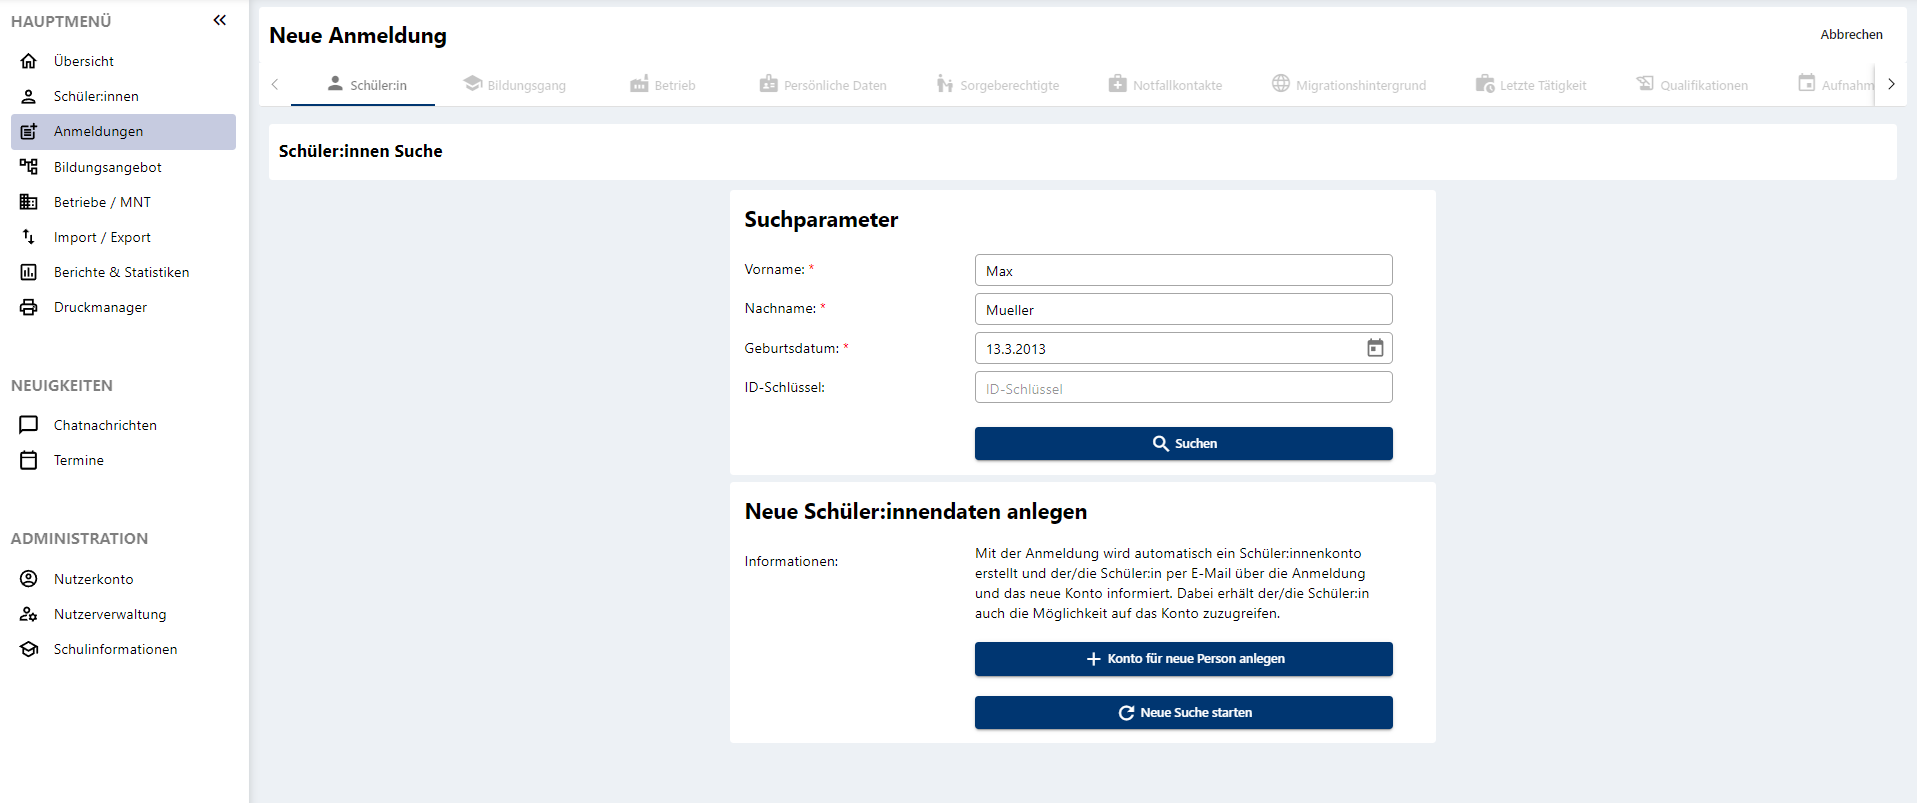
\includegraphics{schuelersuche}
        \end{adjustbox}
    \end{figure}

    \subsection{Screenshot des Tabs \textit{Bildungsgang}}
    \label{section-bildungsgang}
    \begin{figure}[H]
        \centering
        \caption{Testüberschrift}
        \begin{adjustbox}{width=\linewidth, center}
            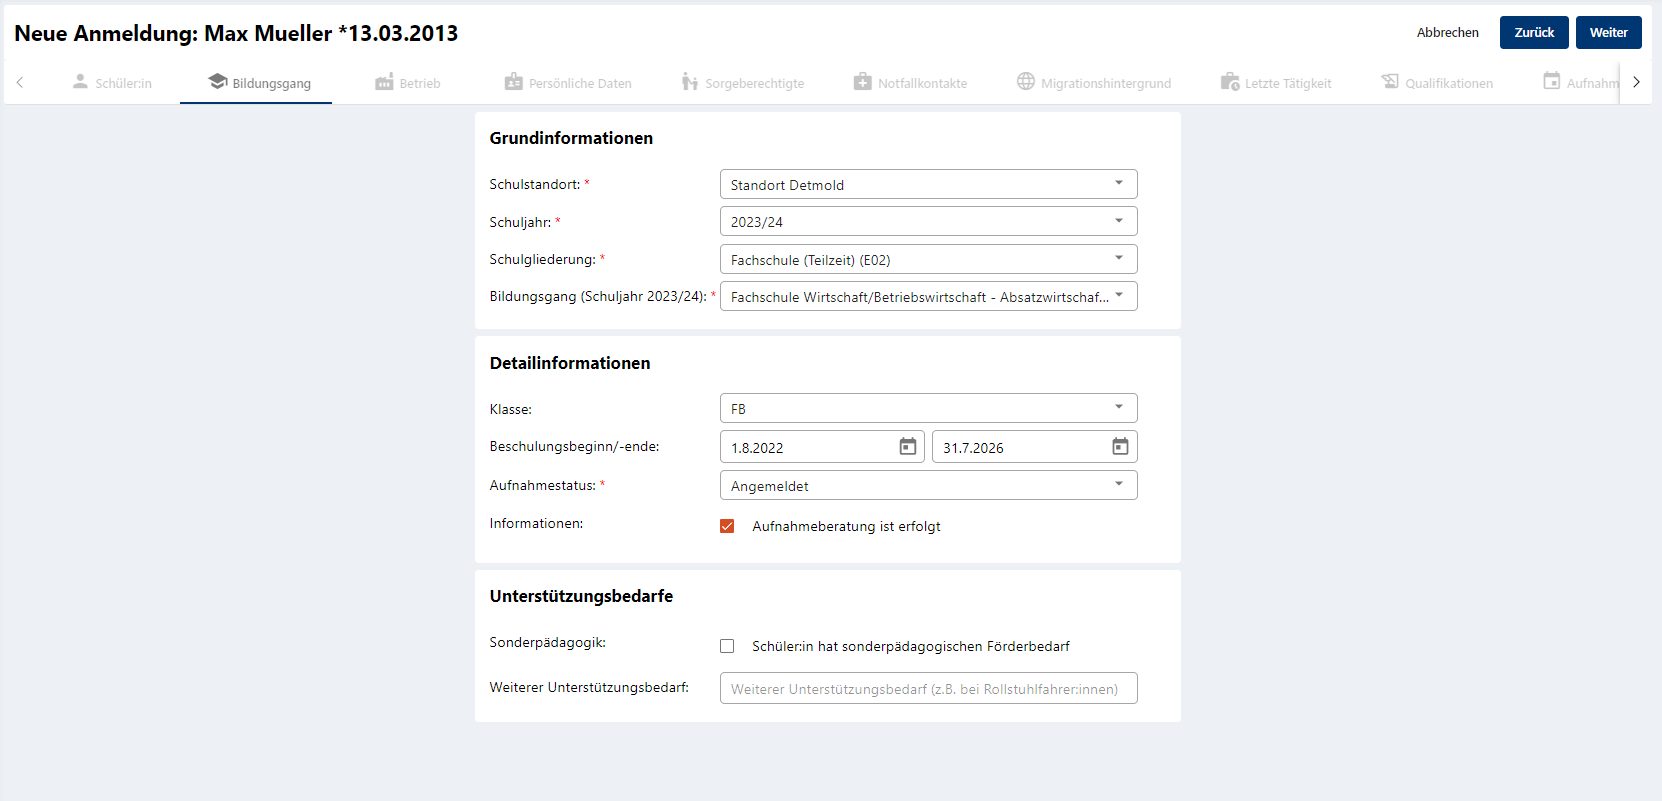
\includegraphics{bildungsgang}
        \end{adjustbox}
    \end{figure}

    \subsection{Screenshot des Tabs \textit{Persönliche Daten}}
    \label{section-persoenliche-daten}
    \begin{figure}[H]
        \centering
        \caption{Testüberschrift}
        \begin{adjustbox}{width=\linewidth, center}
            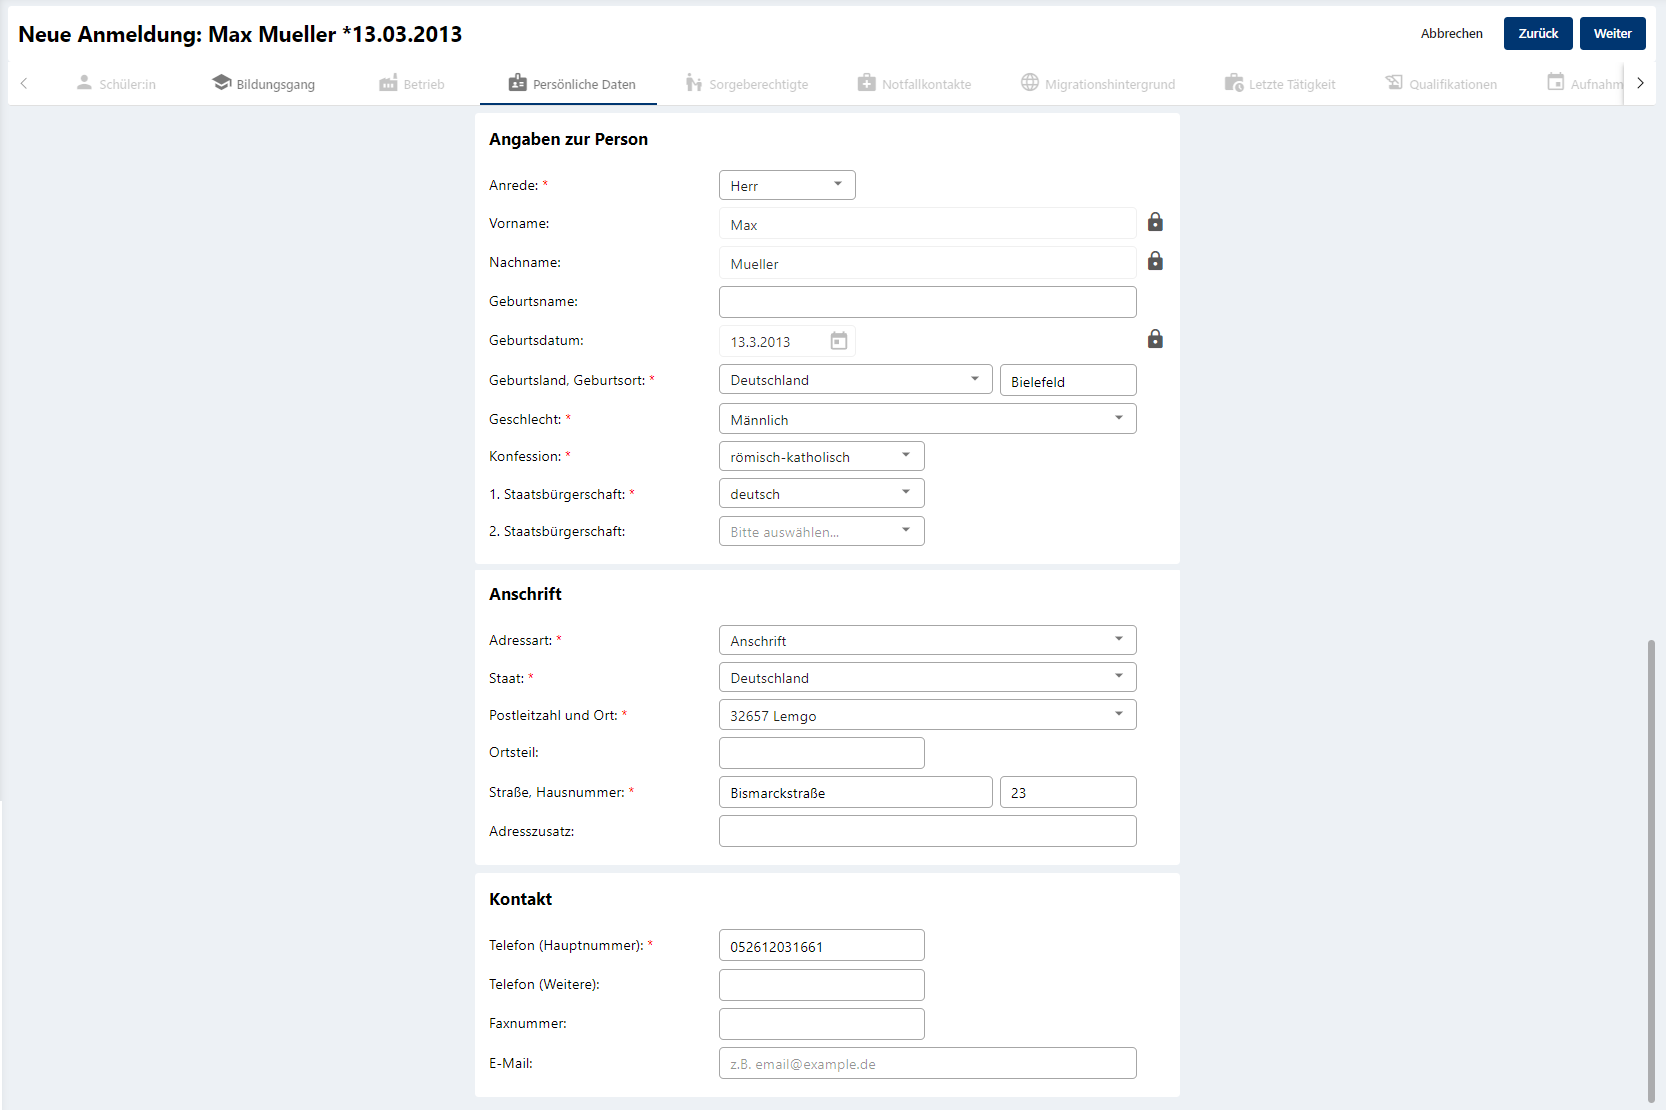
\includegraphics{persoenliche-daten}
        \end{adjustbox}
    \end{figure}

    \subsection{Screenshot des Tabs \textit{Sorgeberechtigte-liste}}
    \label{section-sorgeberechtigte-liste}
    \begin{figure}[H]
        \centering
        \caption{Testüberschrift}
        \begin{adjustbox}{width=\linewidth, center}
            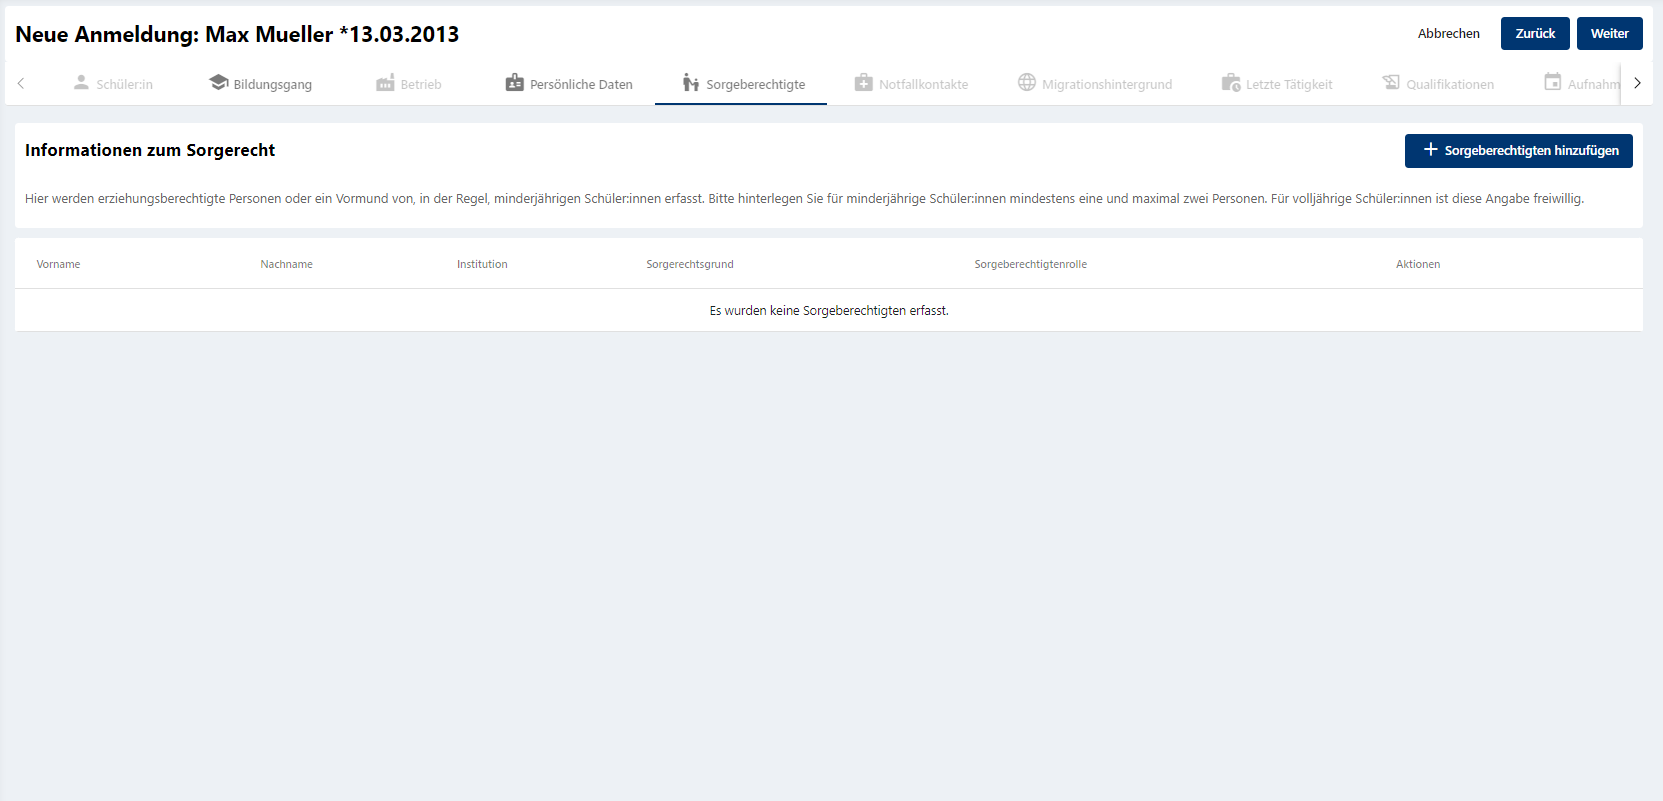
\includegraphics{sorgeberechtigte-liste}
        \end{adjustbox}
    \end{figure}

    \subsection{Screenshot des Tabs \textit{Sorgeberechtigter-person}}
    \label{section-sorgeberechtigter-person}
    \begin{figure}[H]
        \centering
        \caption{Testüberschrift}
        \begin{adjustbox}{width=0.5\linewidth, center}
            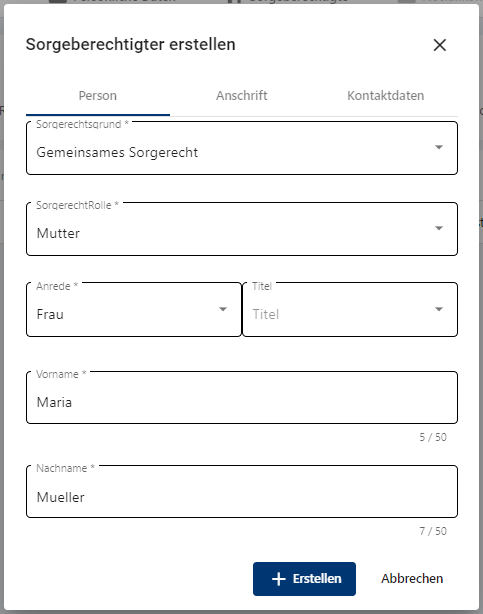
\includegraphics{sorgeberechtigter-person}
        \end{adjustbox}
    \end{figure}

    \subsection{Screenshot des Tabs \textit{Sorgeberechtigter-anschrift}}
    \label{section-sorgeberechtigter-anschrift}
    \begin{figure}[H]
        \centering
        \caption{Testüberschrift}
        \begin{adjustbox}{width=0.85\linewidth, center}
            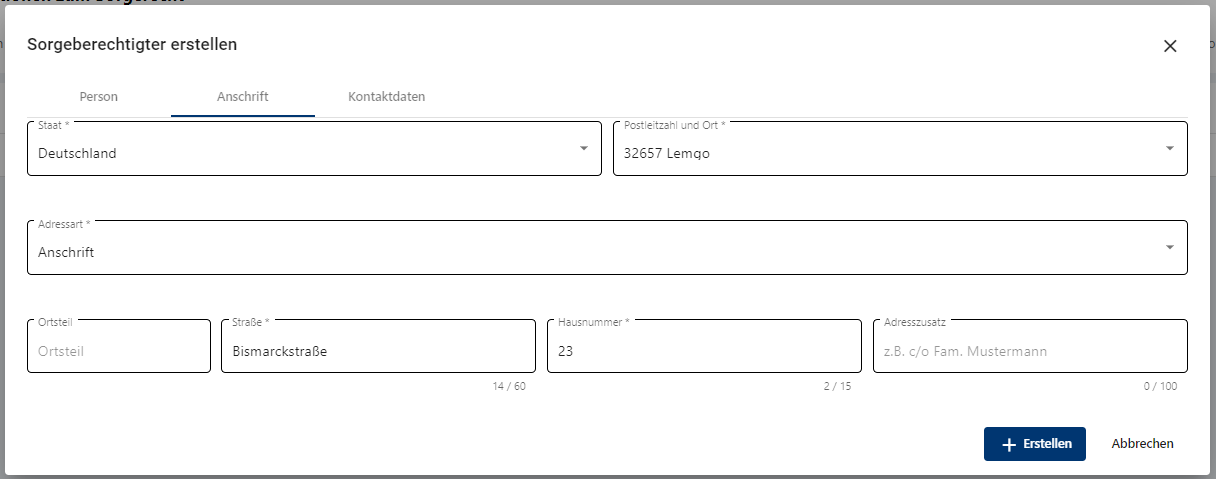
\includegraphics{sorgeberechtigter-anschrift}
        \end{adjustbox}
    \end{figure}

    \subsection{Screenshot des Tabs \textit{Sorgeberechtigter-kontakt}}
    \label{section-sorgeberechtigter-kontakt}
    \begin{figure}[H]
        \centering
        \caption{Testüberschrift}
        \begin{adjustbox}{width=0.6\linewidth, center}
            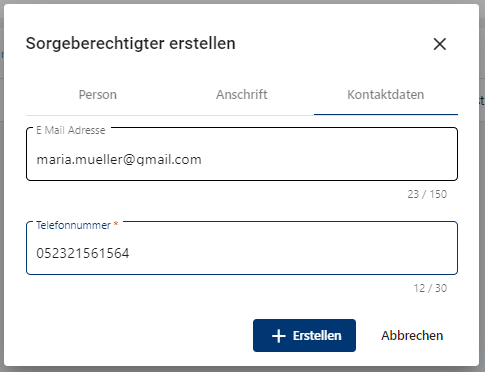
\includegraphics{sorgeberechtigter-kontakt}
        \end{adjustbox}
    \end{figure}

    \subsection{Screenshot des Tabs \textit{Notfallkontakt-liste}}
    \label{section-notfallkontakt-liste}
    \begin{figure}[H]
        \centering
        \caption{Testüberschrift}
        \begin{adjustbox}{width=\linewidth, center}
            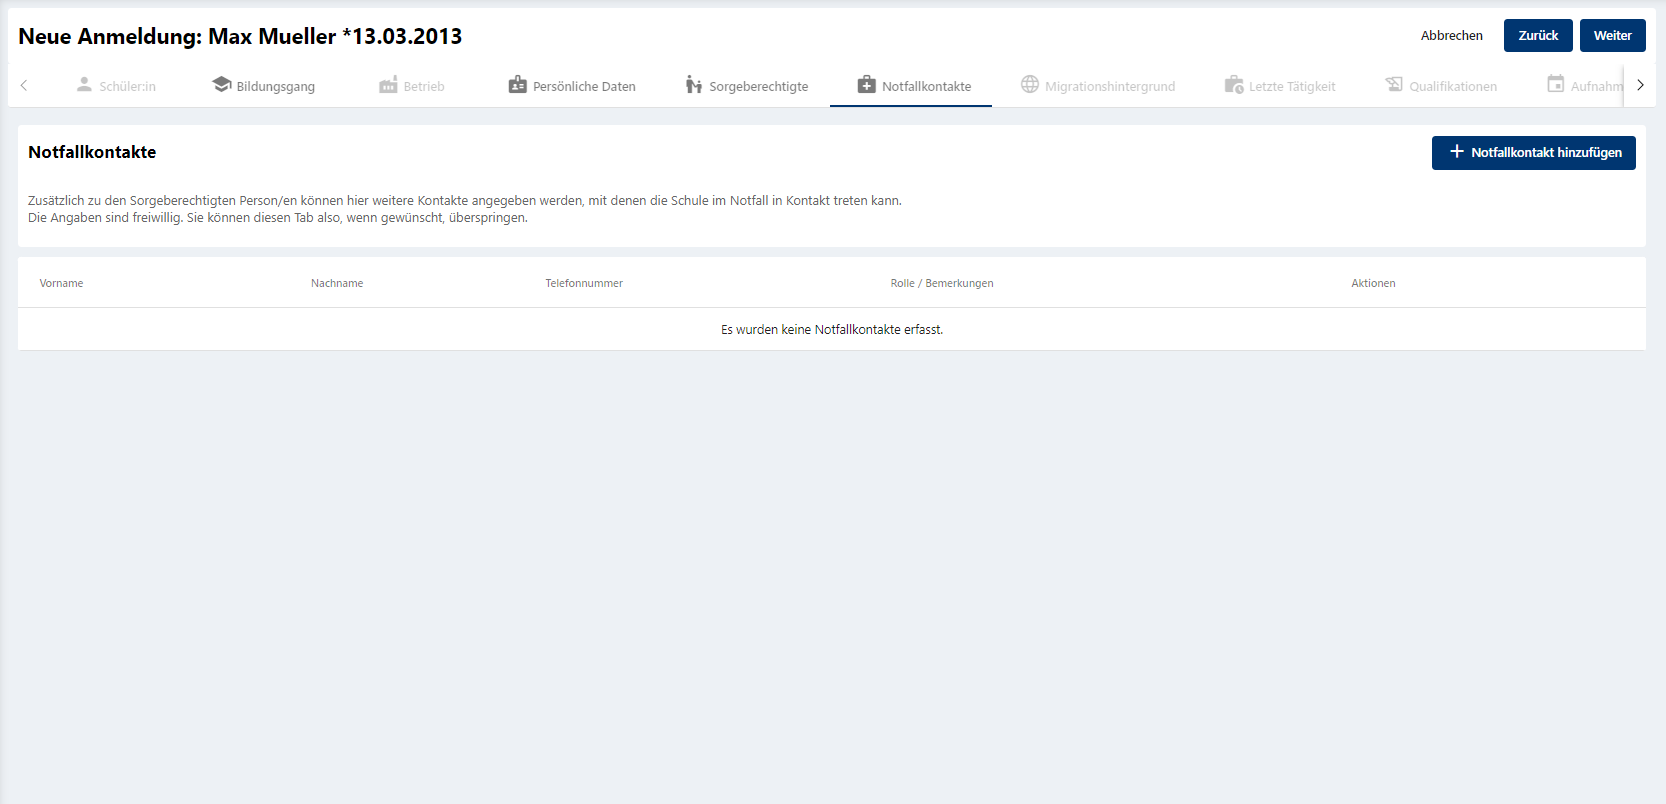
\includegraphics{notfallkontakt-liste}
        \end{adjustbox}
    \end{figure}

    \subsection{Screenshot des Tabs \textit{Notfallkontakt-daten}}
    \label{section-notfallkontakt-daten}
    \begin{figure}[H]
        \centering
        \caption{Testüberschrift}
        \begin{adjustbox}{width=0.6\linewidth, center}
            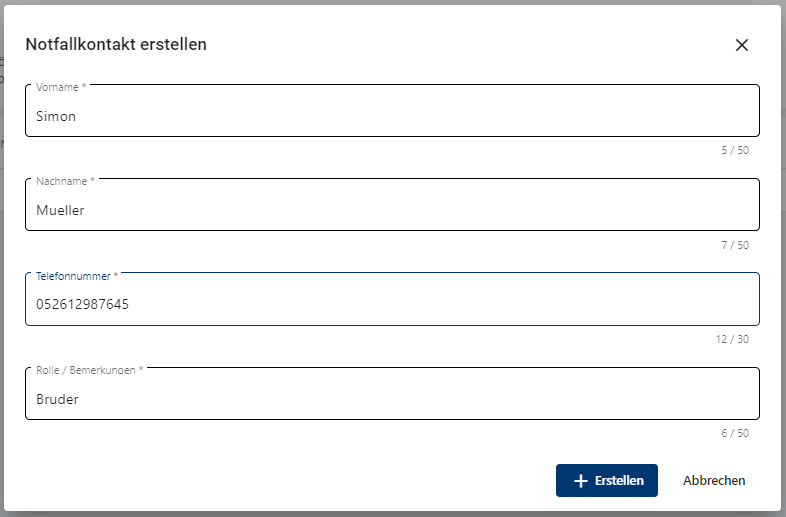
\includegraphics{notfallkontakt-daten}
        \end{adjustbox}
    \end{figure}

    \subsection{Screenshot des Tabs \textit{Migrationshintergrund-liegtvor}}
    \label{section-migrationshintergrund-liegtvor}
    \begin{figure}[H]
        \centering
        \caption{Testüberschrift}
        \begin{adjustbox}{width=\linewidth, center}
            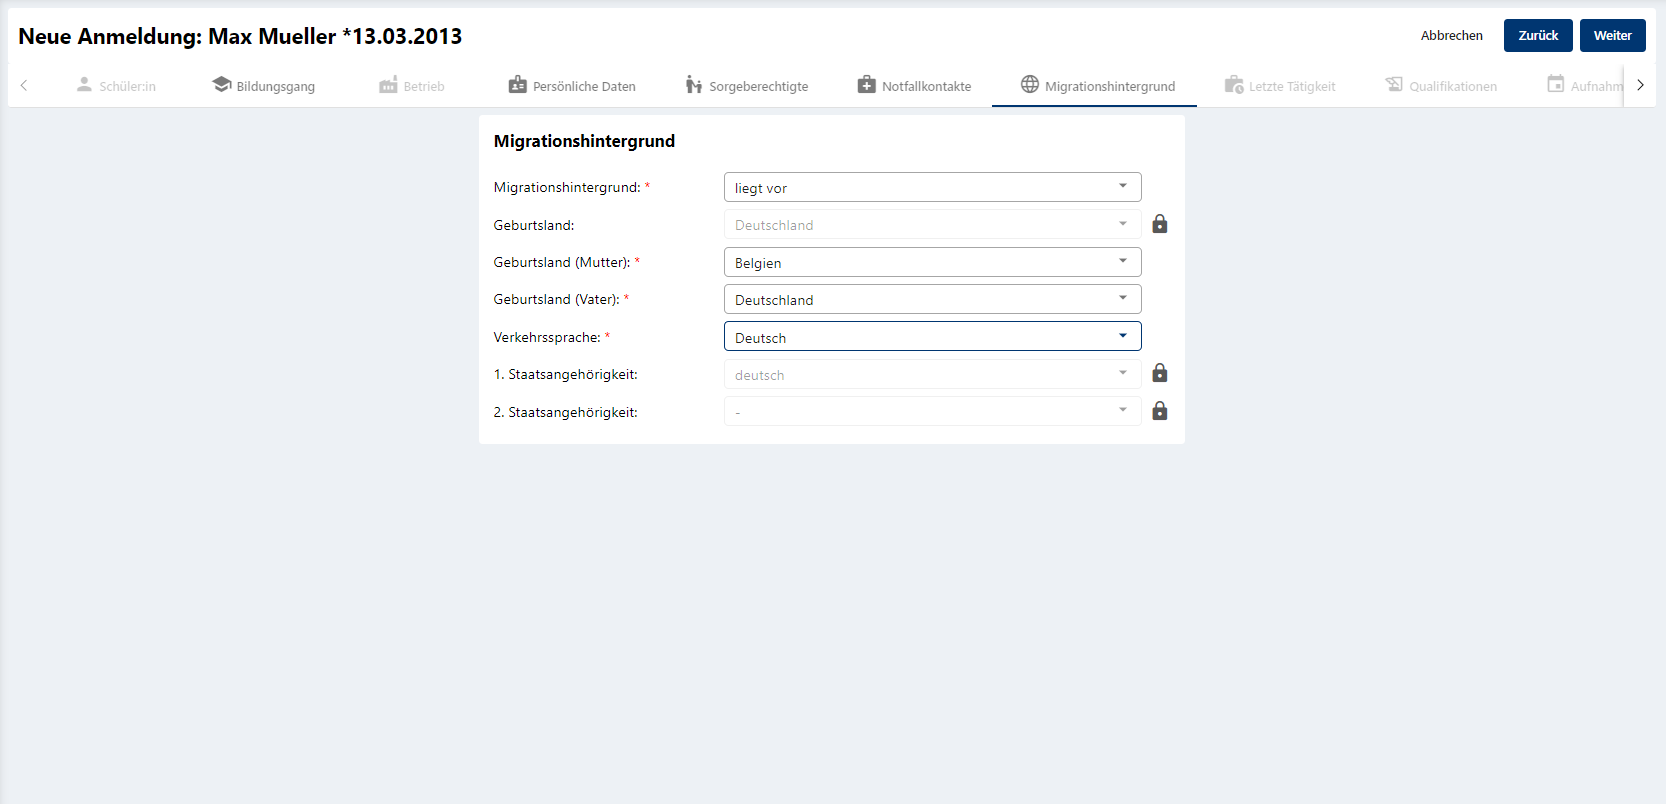
\includegraphics{migrationshintergrund-liegtvor}
        \end{adjustbox}
    \end{figure}

    \subsection{Screenshot des Tabs \textit{Migrationshintergrund-liegtnichtvor}}
    \label{section-migrationshintergrund-liegtnichtvor}
    \begin{figure}[H]
        \centering
        \caption{Testüberschrift}
        \begin{adjustbox}{width=\linewidth, center}
            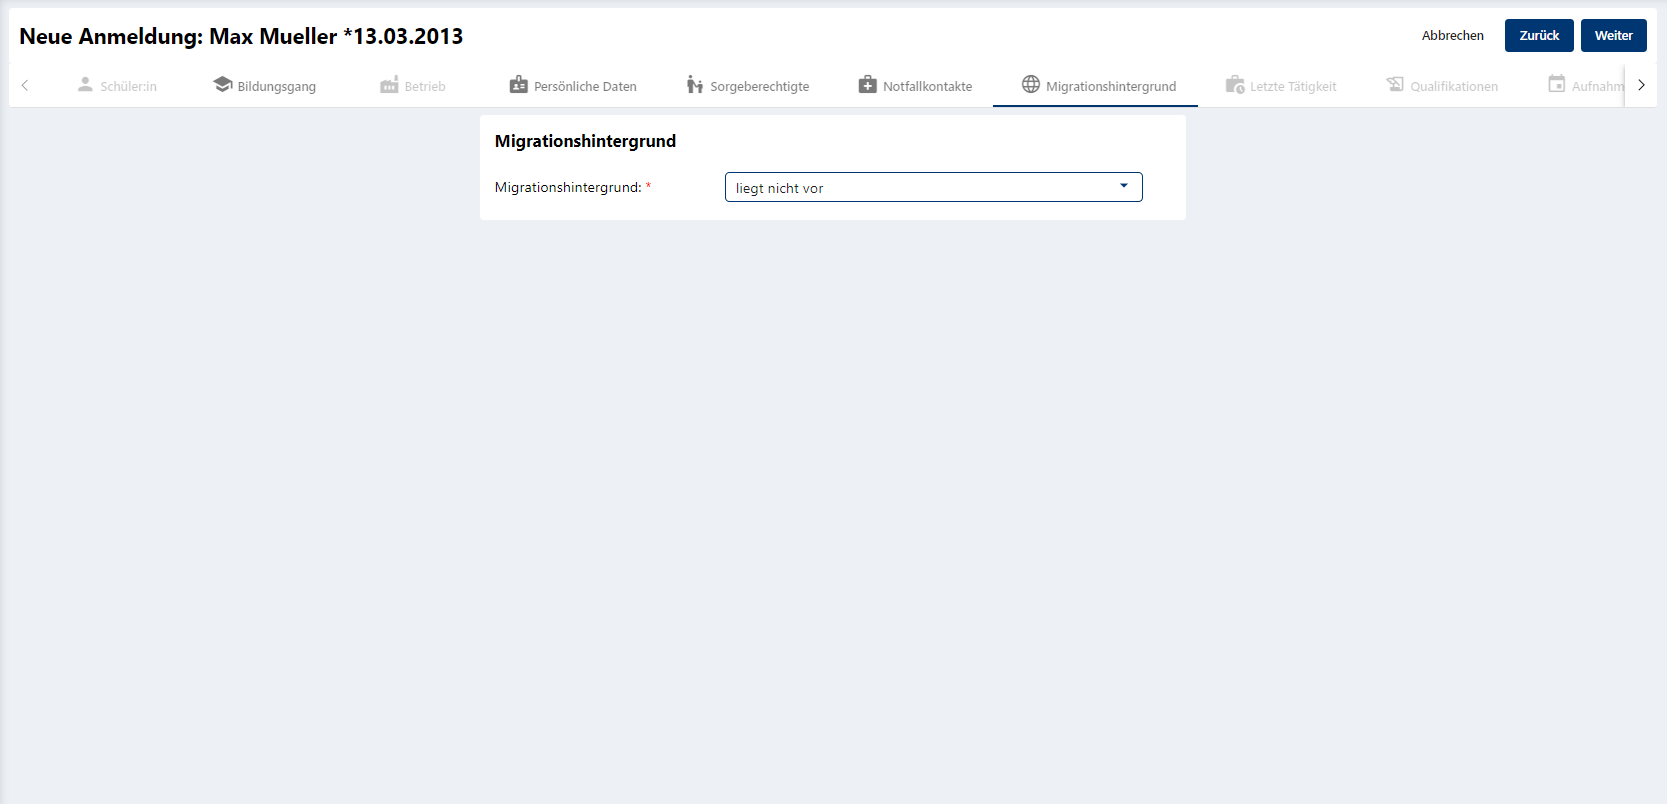
\includegraphics{migrationshintergrund-liegtnichtvor}
        \end{adjustbox}
    \end{figure}

    \subsection{Screenshot des Tabs \textit{Qualifikation}}
    \label{section-qualifikation}
    \begin{figure}[H]
        \centering
        \caption{Testüberschrift}
        \begin{adjustbox}{width=\linewidth, center}
            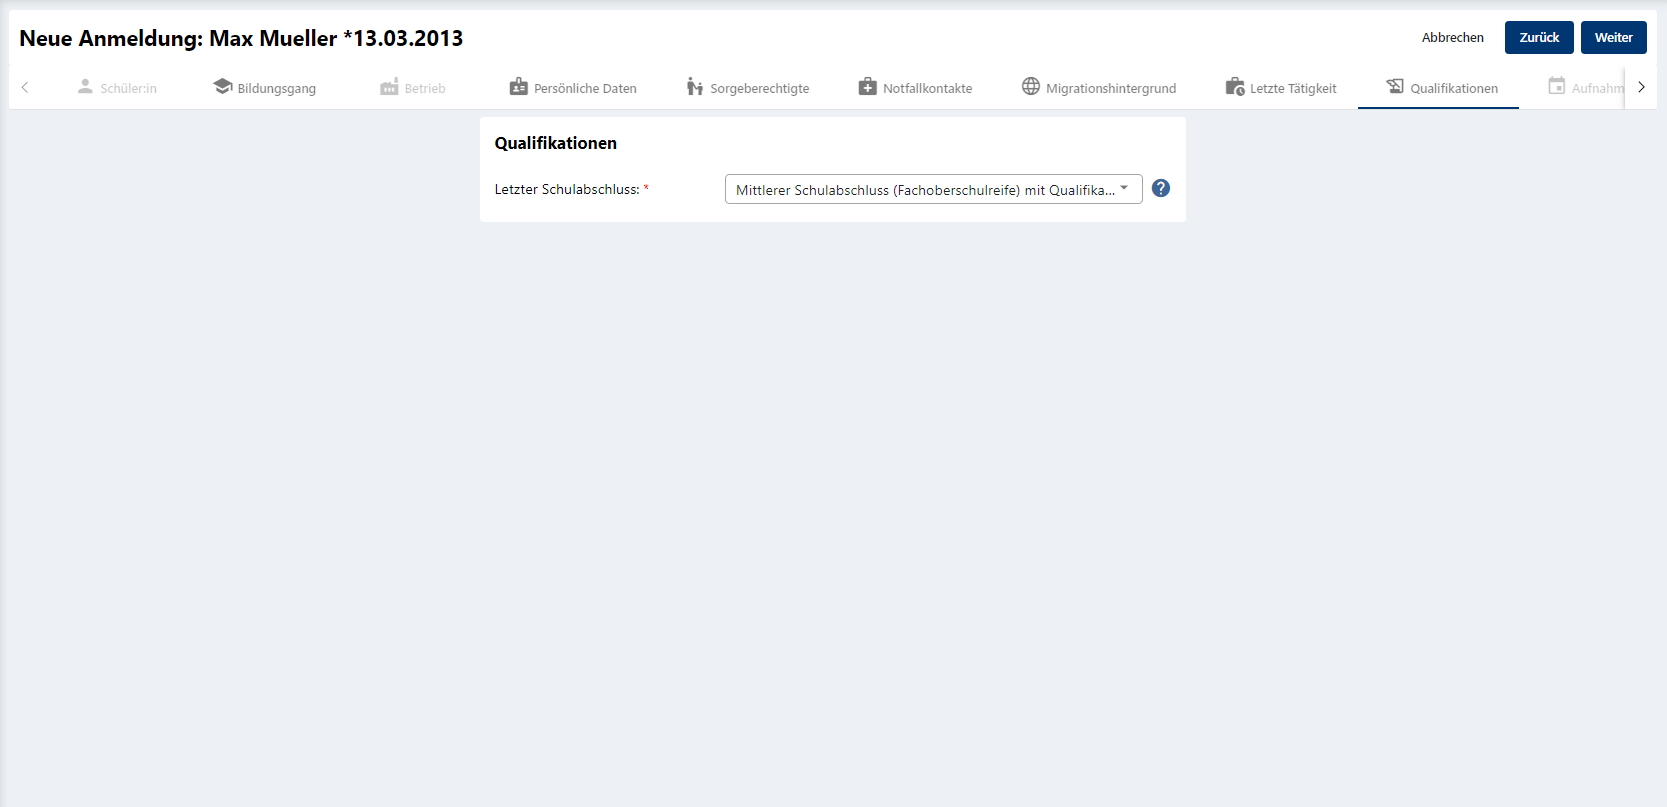
\includegraphics{qualifikation}
        \end{adjustbox}
    \end{figure}

    \subsection{Screenshot des Tabs \textit{Letztetaetigkeit}}
    \label{section-letztetaetigkeit}
    \begin{figure}[H]
        \centering
        \caption{Testüberschrift}
        \begin{adjustbox}{width=\linewidth, center}
            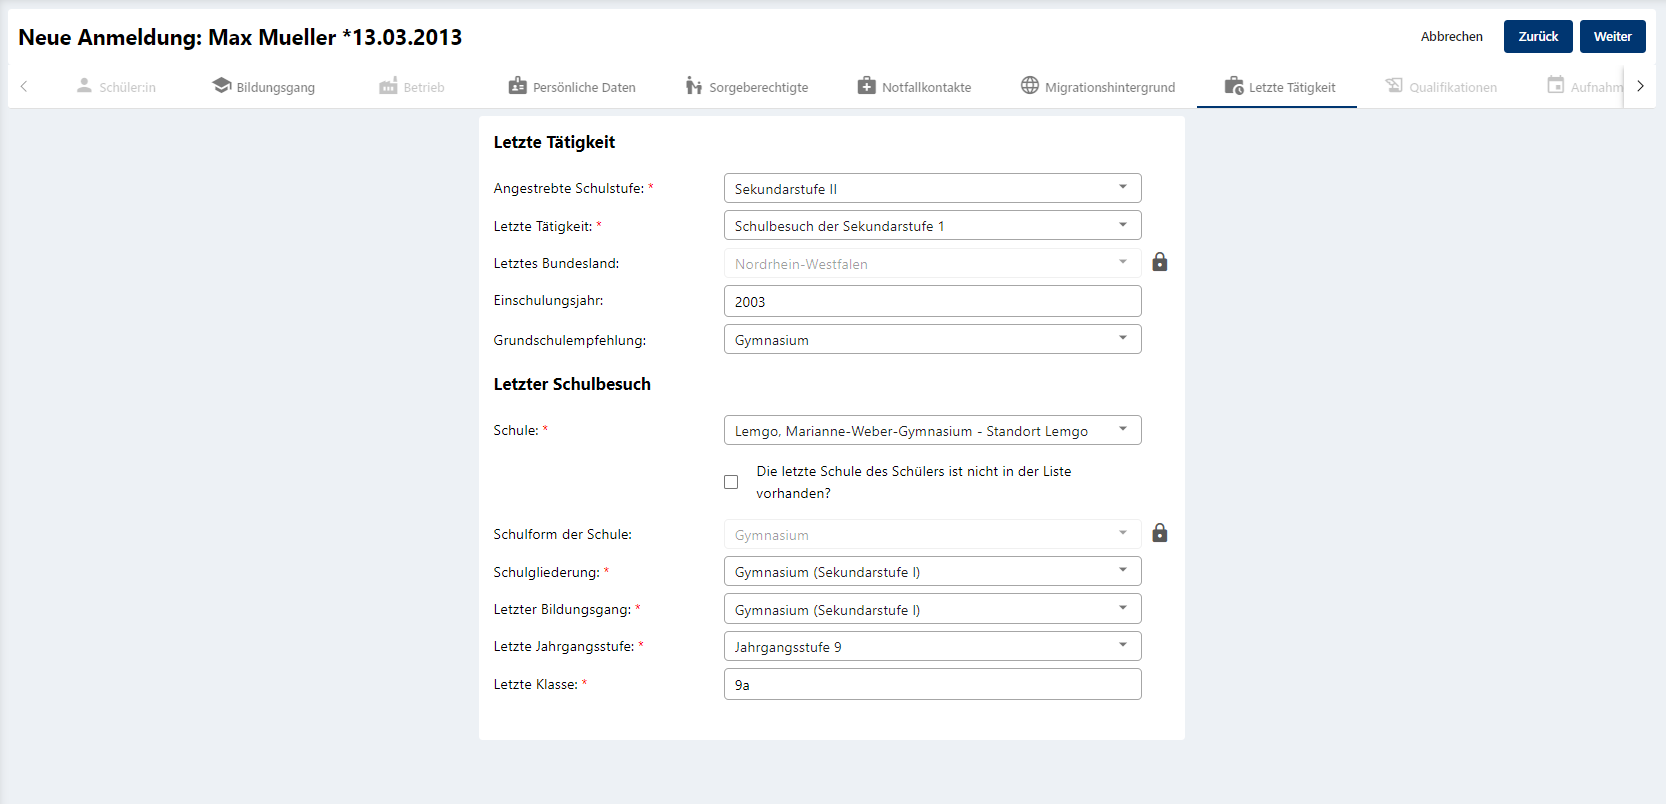
\includegraphics{letztetaetigkeit}
        \end{adjustbox}
    \end{figure}

    \subsection{Screenshot des Tabs \textit{Aufnahmeberatung}}
    \label{section-aufnahmeberatung}
    \begin{figure}[H]
        \centering
        \caption{Testüberschrift}
        \begin{adjustbox}{width=\linewidth, center}
            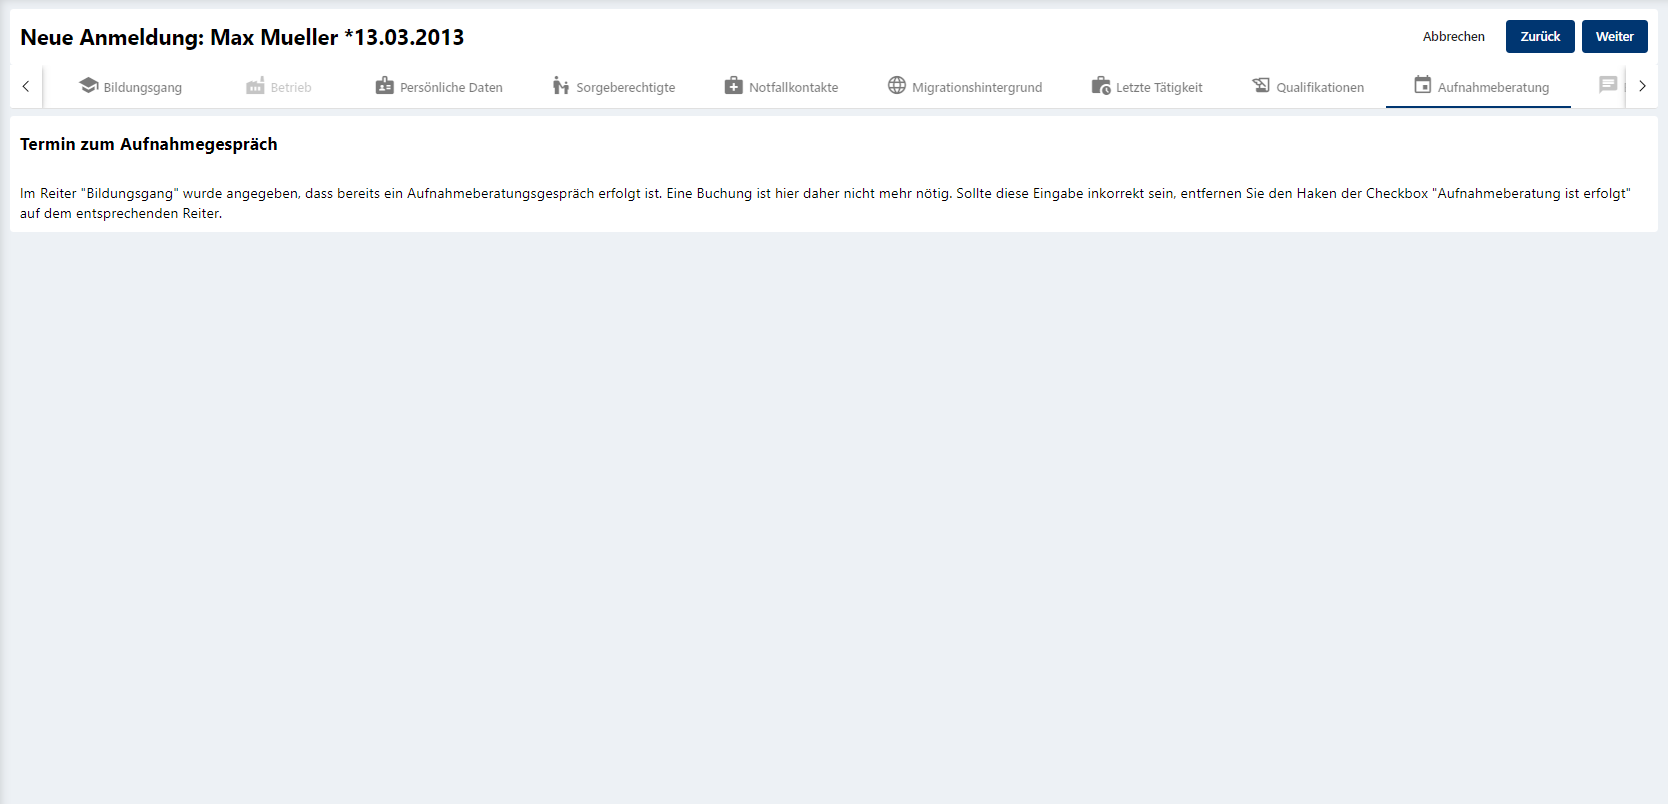
\includegraphics{aufnahmeberatung}
        \end{adjustbox}
    \end{figure}

    \subsection{Screenshot des Tabs \textit{Bemerkungen}}
    \label{section-bemerkungen}
    \begin{figure}[H]
        \centering
        \caption{Testüberschrift}
        \begin{adjustbox}{width=\linewidth, center}
            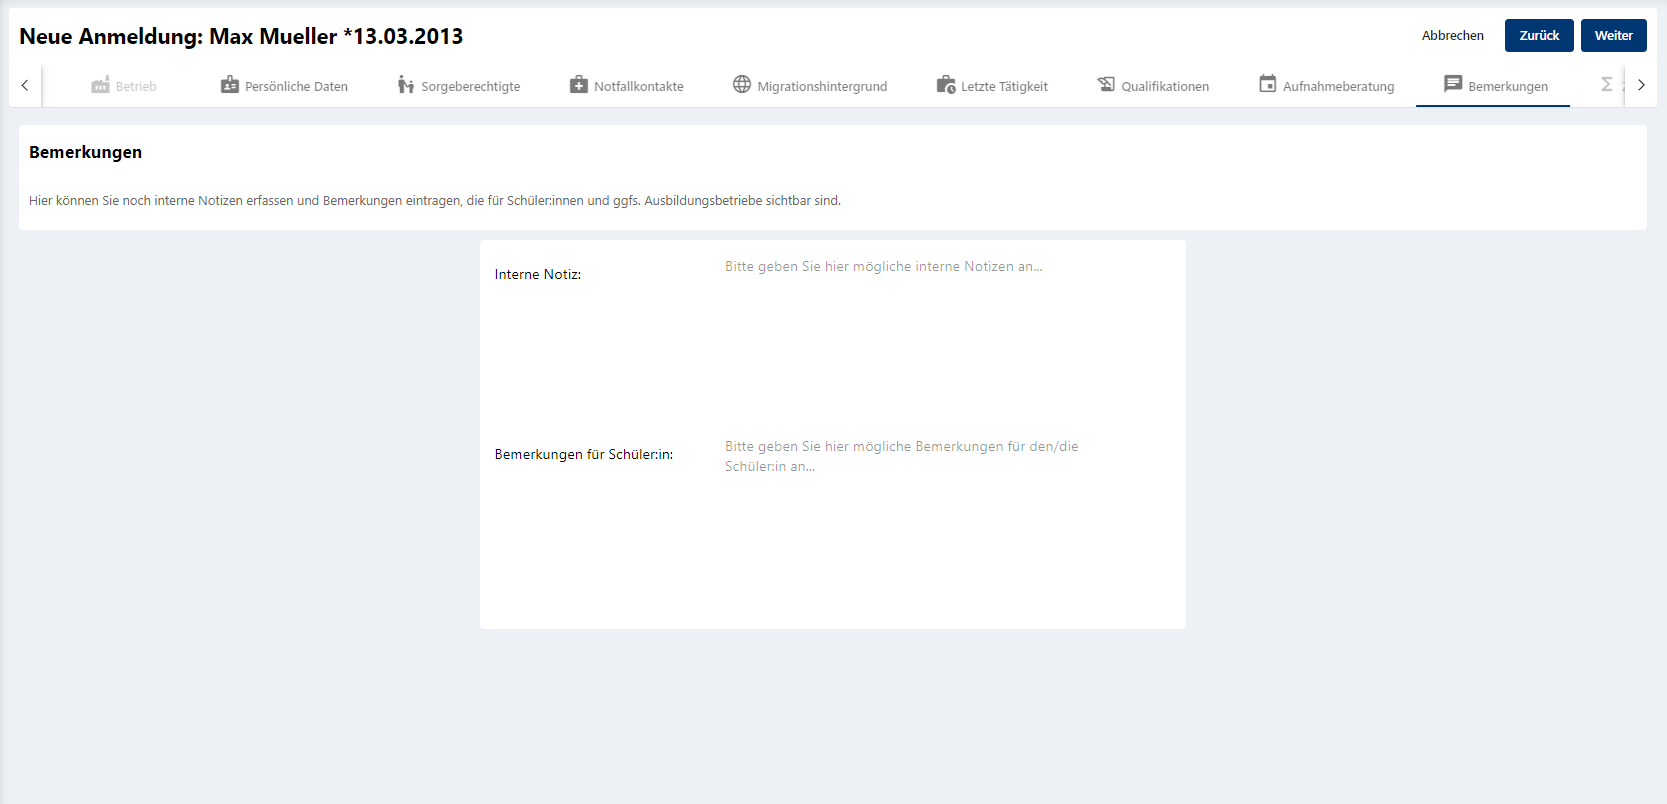
\includegraphics{bemerkungen}
        \end{adjustbox}
    \end{figure}

    \subsection{Screenshot des Tabs \textit{Zusammenfassung}}
    \label{section-zusammenfassung}
    \begin{figure}[H]
        \centering
        \caption{Testüberschrift}
        \begin{adjustbox}{width=\linewidth, center}
            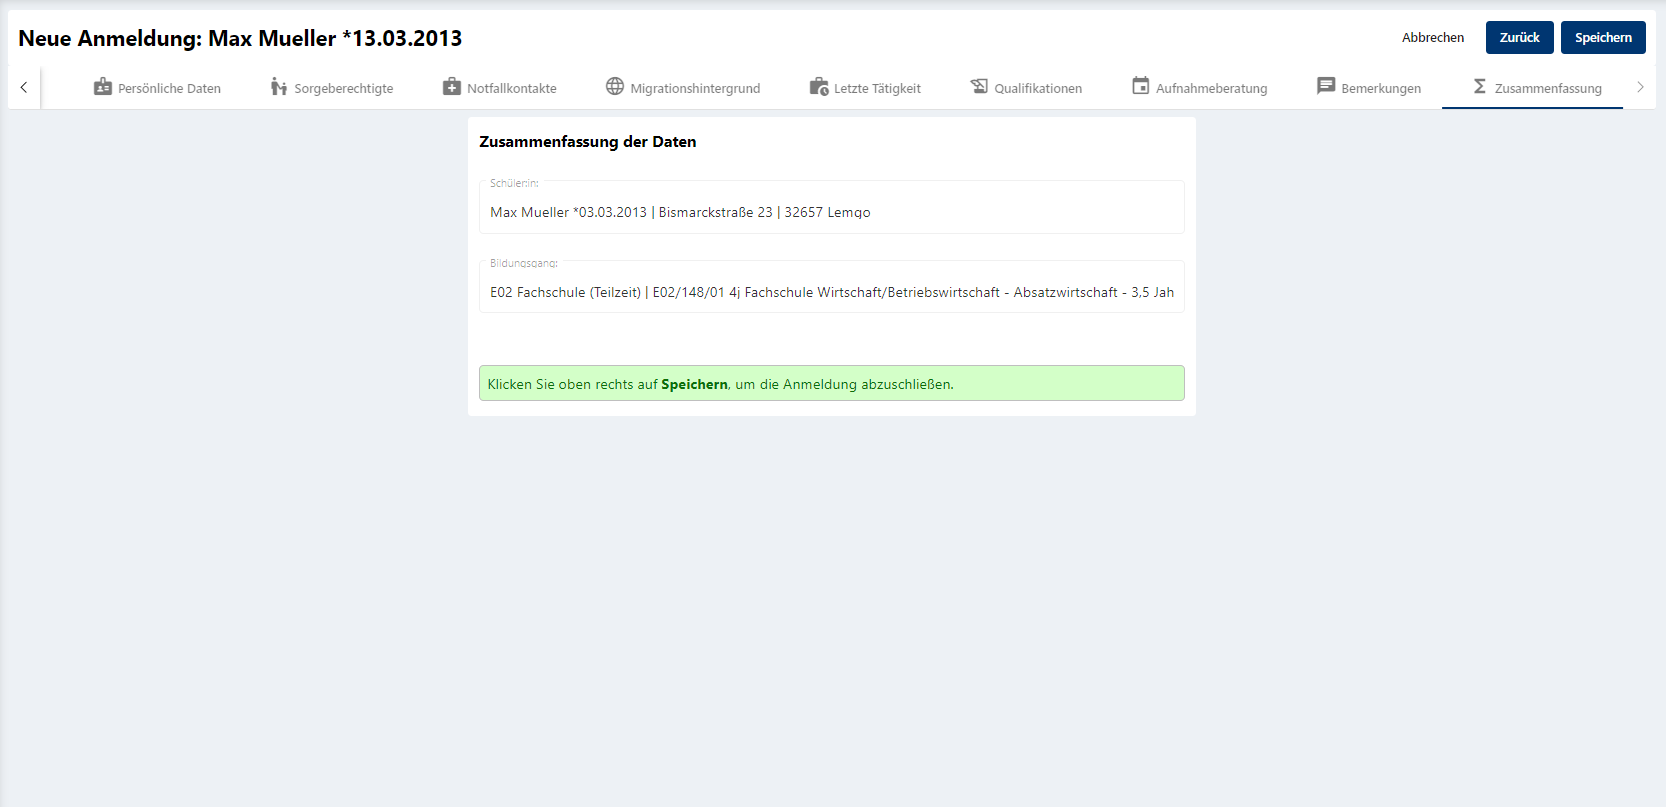
\includegraphics{zusammenfassung}
        \end{adjustbox}
    \end{figure}

    \subsection{Screenshot des Tabs \textit{Bestaetigung}}
    \label{section-bestaetigung}
    \begin{figure}[H]
        \centering
        \caption{Testüberschrift}
        \begin{adjustbox}{width=\linewidth, center}
            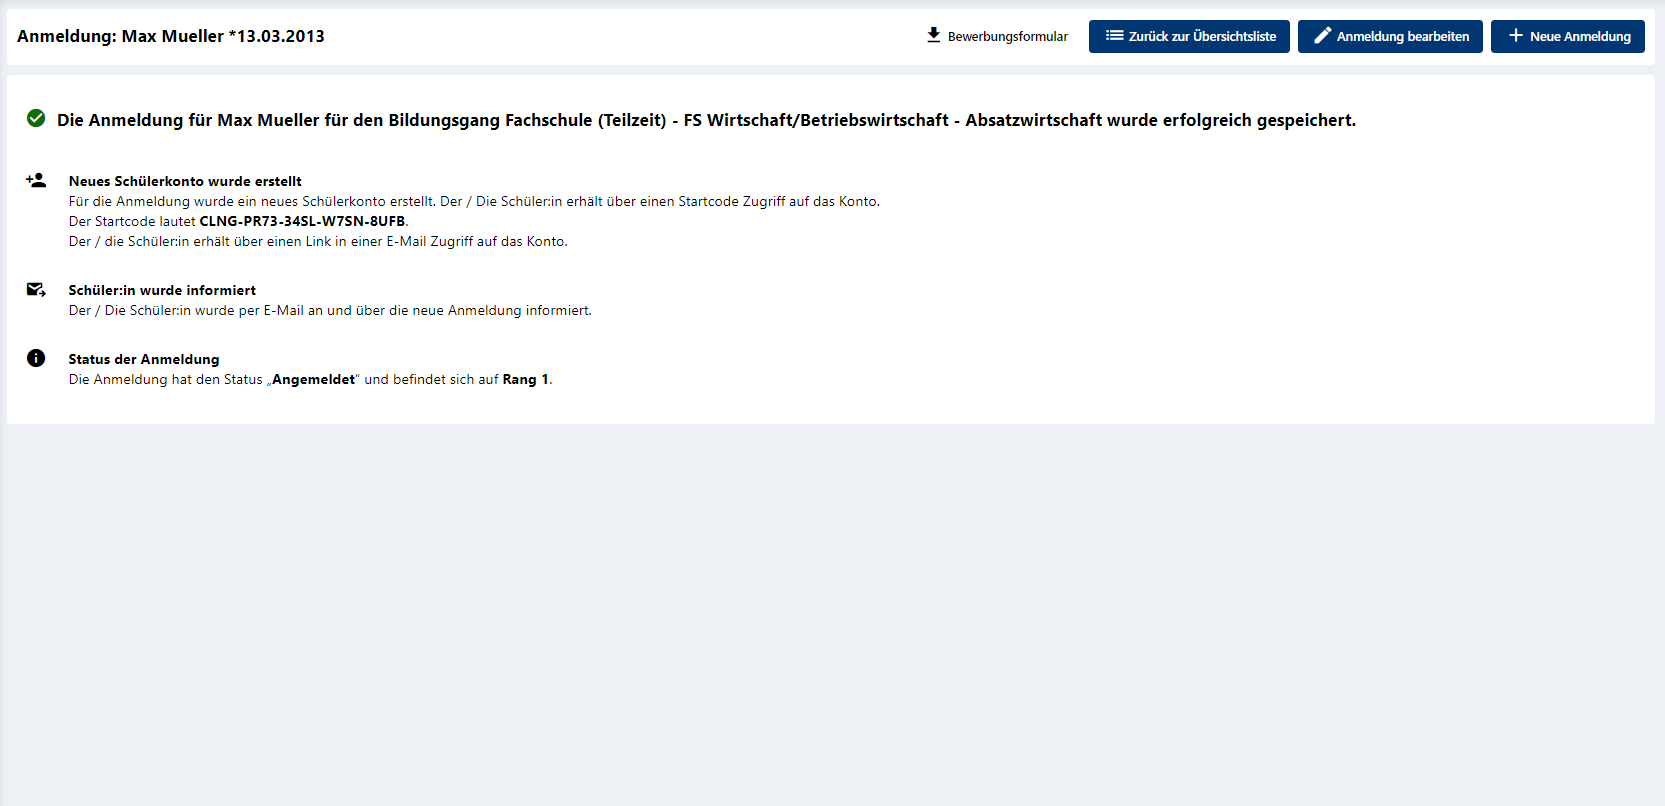
\includegraphics{bestaetigung}
        \end{adjustbox}
    \end{figure}

    \subsection{Screenshot des Tabs \textit{Anmeldung} im Update Prozess}
    \label{section-update-anmeldung}
    \begin{figure}[H]
        \centering
        \caption{Testüberschrift}
        \begin{adjustbox}{width=\linewidth, center}
            \includegraphics{update-anmeldung}
        \end{adjustbox}
    \end{figure}

\end{landscape}
